\chapter{The Effects of Linked Selection.}

\newthought{Genetic drift is not the only source of randomness} in the dynamics of
alleles. Alleles also experience random fluctuations in frequency due to
the fact that they are present on a set of random genetic backgrounds with
different fitnesses. For example, when a beneficial allele arises via a single mutation, it arises on
a particular genetic background, i.e. a particular haplotype (Figure \ref{fig:HIV_sweep}}A). Imagine this mutation arising in a region with no recombination, or in an
organism where genetic exchange is rare. If our beneficial allele
becomes established in the population, i.e. escapes loss by genetic
drift in those first few generations, it will start to increase in
frequency rapidly. As it rises in frequency, so will the alleles that happened to
be present on the haplotype that the mutation arose on (if those
other alleles are neutral or at least not too deleterious). These
other alleles are getting to 'hitchhike' along \citep{}. The alleles that are
not on that particular background are swept out of the population, so the net effect
of this selective sweep is to remove genetic diversity from the
population. Diversity will eventually recover, as new mutations
arise and some slowly drift up in frequency. But in the
short-term, selective sweeps remove genetic variation from
populations. 

\begin{figure}
\begin{center}
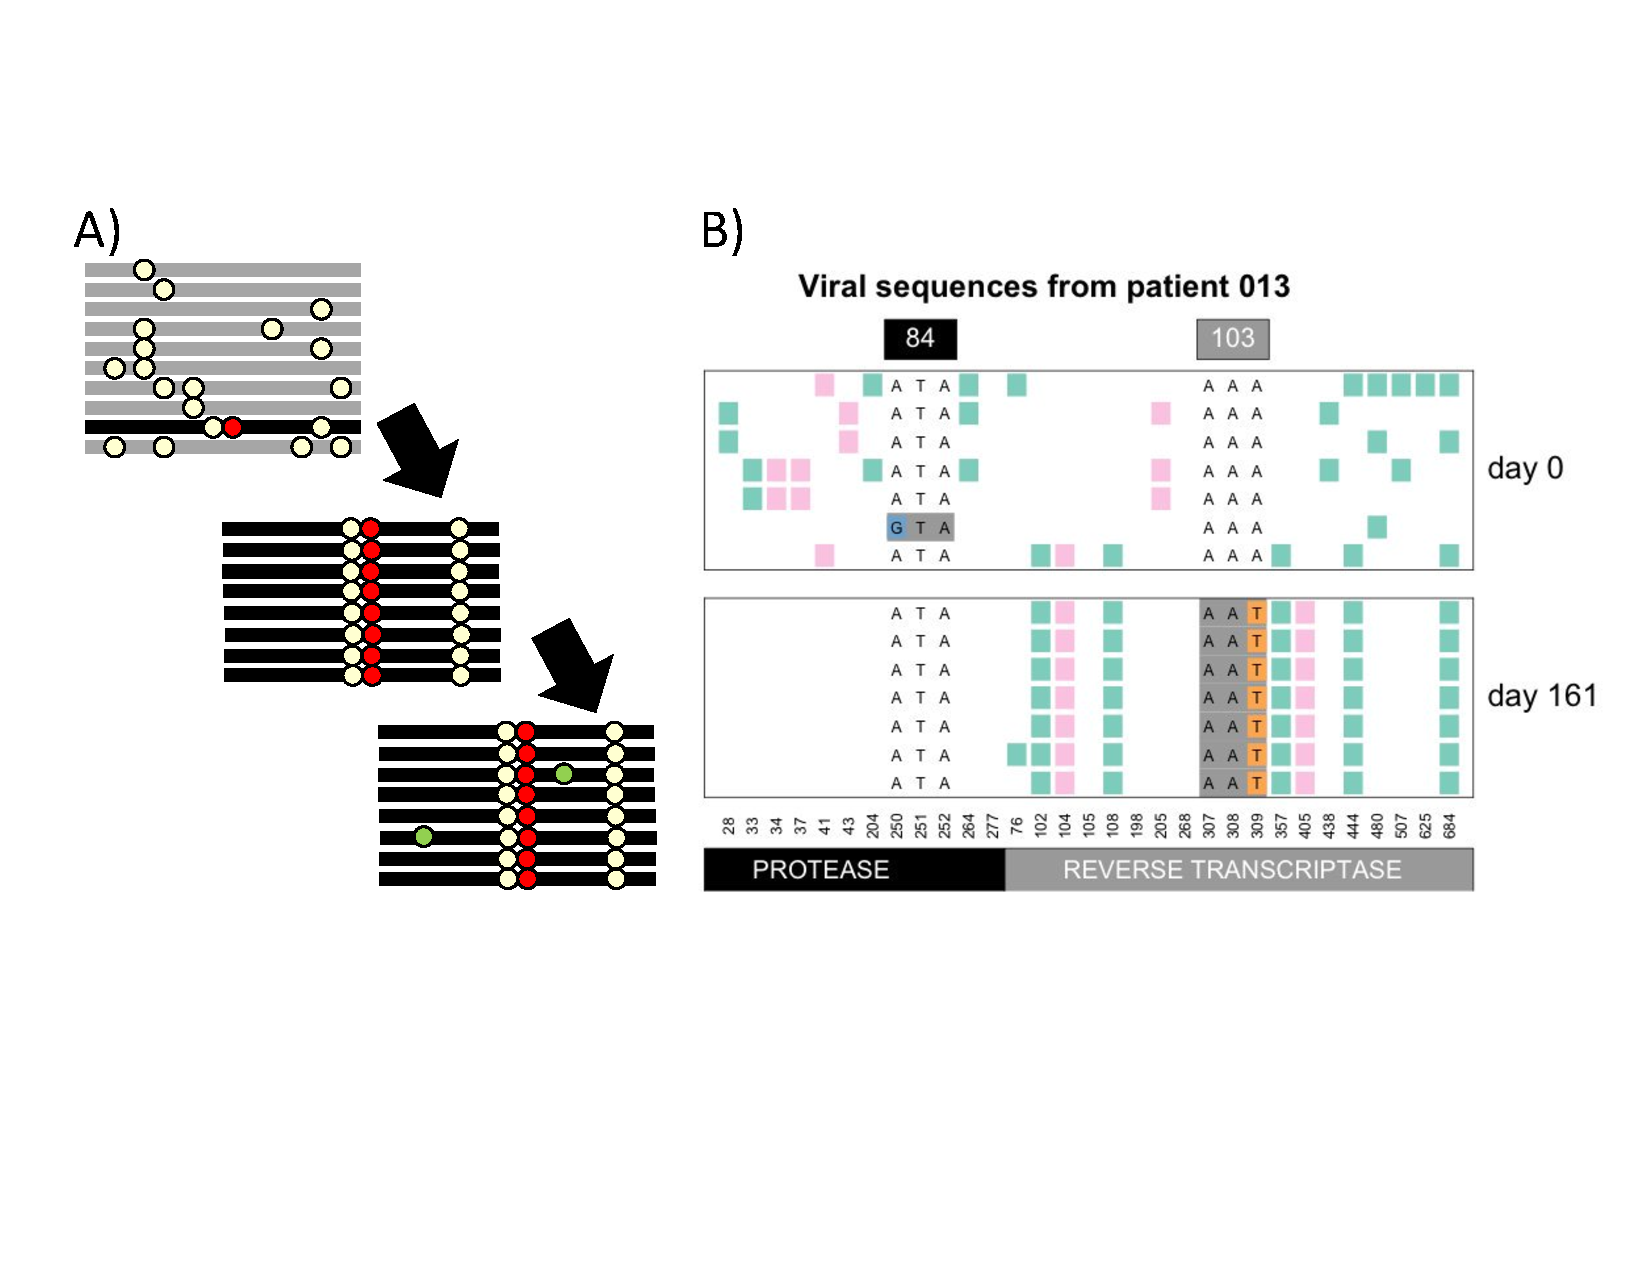
\includegraphics[width= \textwidth]{Journal_figs/recom_selection/Pleuni_HIV_sweep/HIV_no_recom_sweep.pdf}
\end{center}
\caption[][-2cm]{{\bf A)} In the top panel, a selected mutation (red dot) arises
on a particular haplotype in the population. It sweeps to fixation,
carrying with it the haplotype on which it arose, middle panel,
erasing the standing genetic diversity in the region. The bottom panel
is some time after the selective sweep when some new neutral alleles (green
dots) have started to drift up in frequency. {\bf B)}  Top panel: HIV
sequences from a patient at the start of drug treatment in the
protease and retrotransposase coding regions. Bottom panel: A sample
161 days later, after a drug resistant mutation has spread, the A
$\rightarrow$ T in the $103^{rd}$ codon of retrotransposase. Each row is a haplotype,
with the alleles present shown as coloured blocks. Figure B from
\citet{Williams548198}, \PLOSccBY.} \label{fig:HIV_sweep}  %\hyper{https://github.com/PenningsLab/ClonalInterferenceHIV}{
\end{figure}

\citet{Williams548198} have visualized selective sweeps in
HIV. In Figure \ref{fig:HIV_sweep}B) we see a set of HIV haplotypes
sampled from a patient before and after of a selective sweep of a
drug-resistant mutation. The patient is taking a
retrotransposase inhibitor (Efavirenz), but sadly within 161 days a
drug-resistant mutation that changes the HIV retrotransposase protein has arisen and spread. Note how a particular haplotype is now fixed in
the sample, and little genetic diversity remains, due to the
hitchhiking effect of the strong
selective sweep of this allele. 


\begin{marginfigure}
\begin{center}
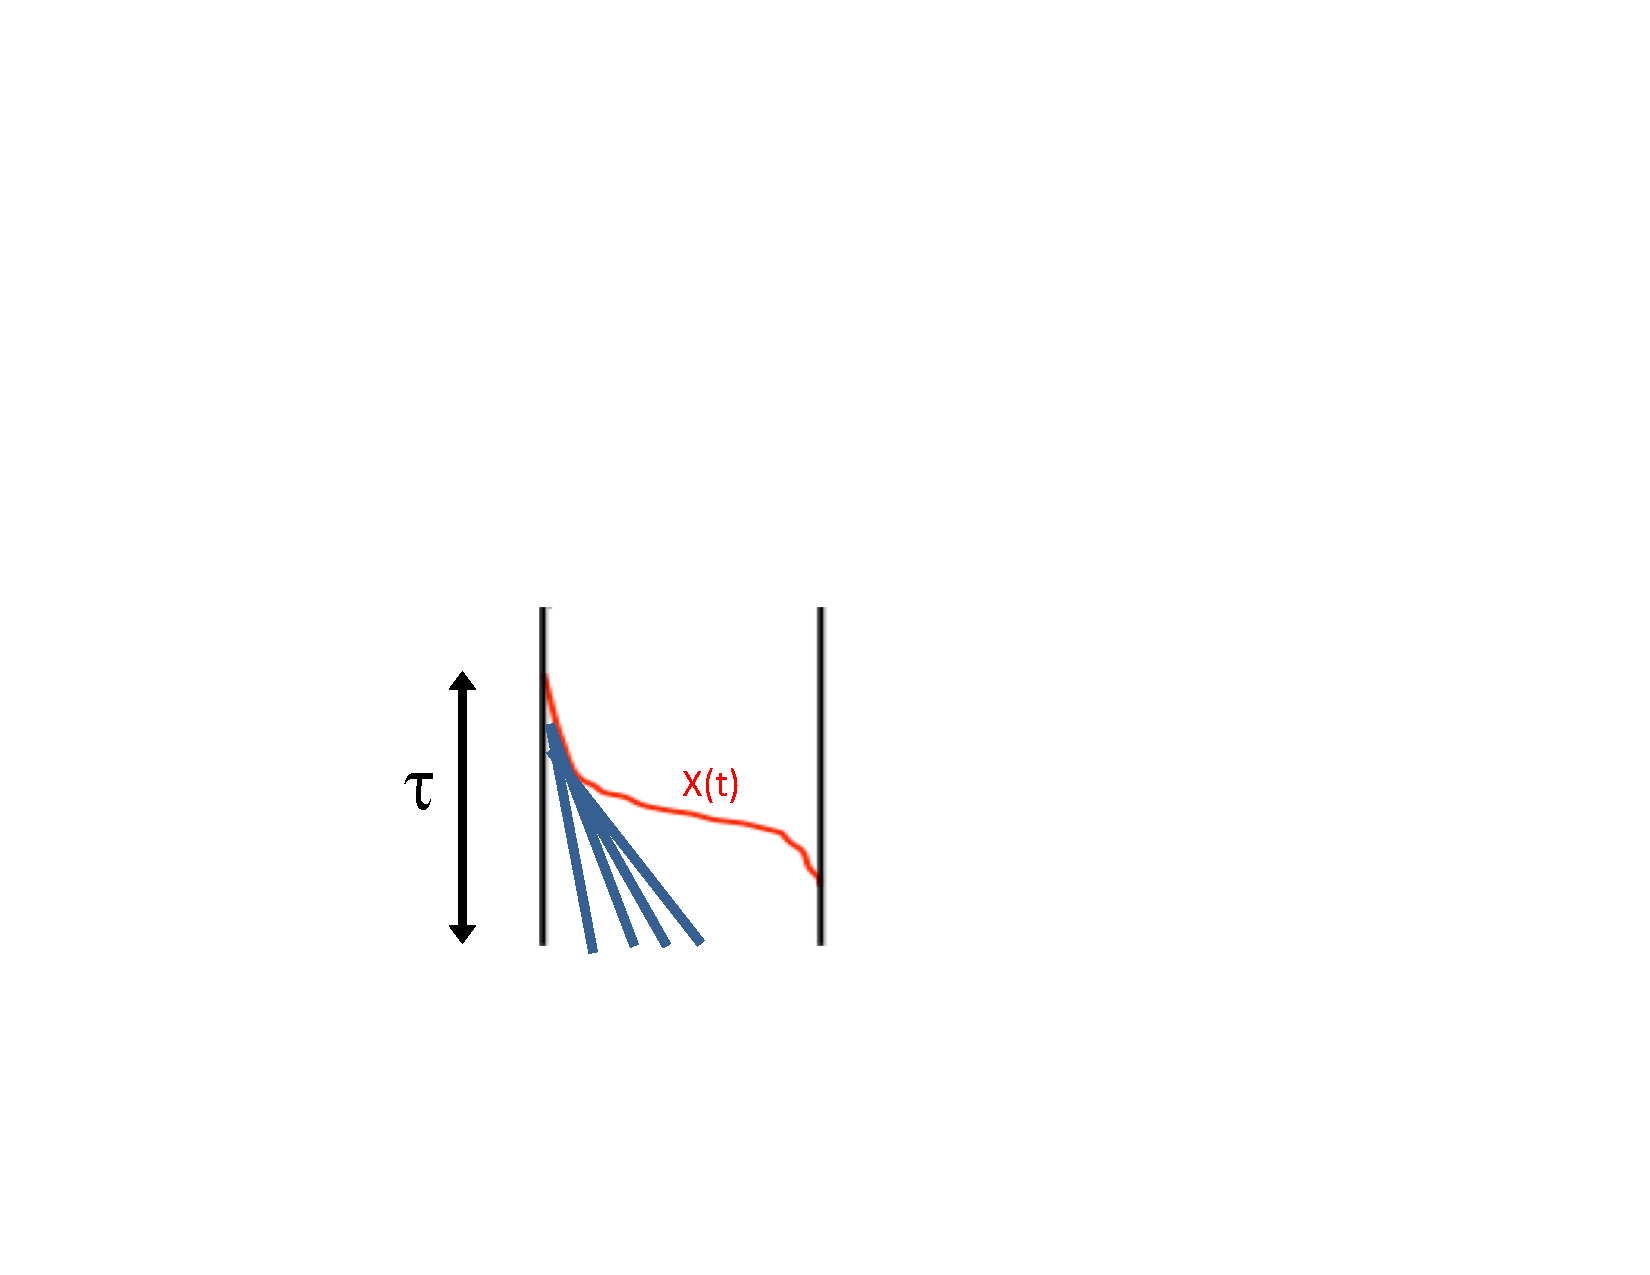
\includegraphics[width= 0.75 \textwidth]{figures/Hitchhiking/No_recom_coal.pdf}
\end{center}
\caption{The coalescent of 4 lineages, marked in blue, at a locus completed linked to our selected allele. The frequency trajectory of the selected allele $X(t)$ is shown in red.} \label{fig:no_recom_coal}
\end{marginfigure}
To better understand hitchhiking, first let's imagine examining variation at a locus fully linked
to our selected locus, just after our sweep reached fixation. Neutral alleles sampled at this locus
must trace their ancestral lineages back to the neutral
allele on whose background the selected allele initially arose (Figure
\ref{fig:no_recom_coal}). This is because
that background neutral allele, which existed $\tau$ generations ago, is the
ancestor of the entire population at this fully linked locus. Our individuals who
carry the beneficial allele are, from the perspective of these 
alleles, experiencing a rapidly expanding population. Therefore, a
pair of neutral alleles sampled at our linked neutral locus will be forced to
coalesce $\approx \tau$ generations ago. A newly derived allele with an additive selection coefficient $s$ will
take a time $\tau = 4\log(2N)/s$ generations to reach to fixation
within our population (see eqn. \eqref{eq:diploid_fix_time}). This is a very
short-time scale compared to the average neutral coalescent time of
$2N$ generations for a pair of alleles. Thus we expect little variation,
as few mutations will have arisen on these very short branches, and
those that have done will likely be singletons in our sample. \\

\begin{marginfigure}
\begin{center}
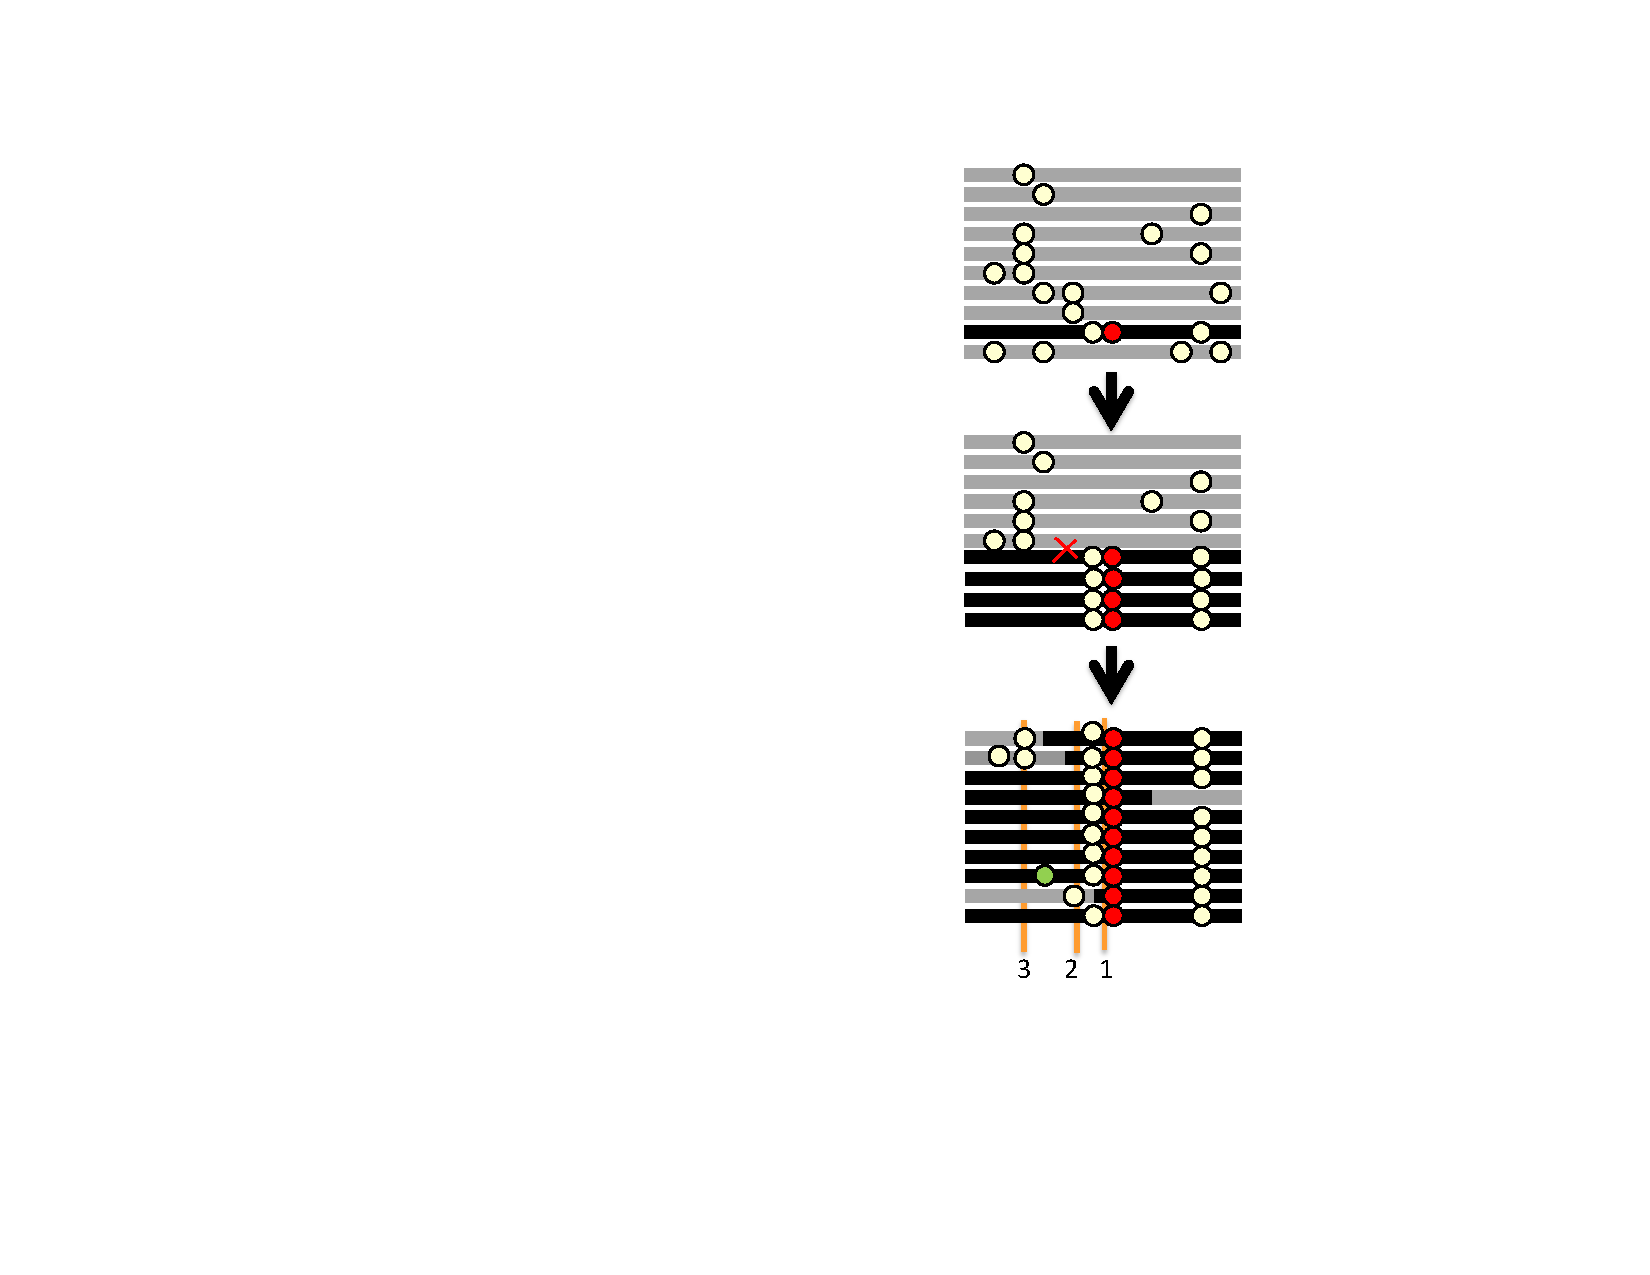
\includegraphics[width= 0.5 \textwidth]{figures/Hitchhiking/recom_haps_sweep.pdf}
\end{center}
\caption{A cartoon depiction of a sweep of a red beneficial allele
  over three time points with recombination. The haplotype that the beneficial arose on by mutation is shown in black. The three vertical orange lines mark the loci shown in Figure \ref{fig:sweep_haps_coal}. Neutral alleles segregating prior to the sweep appear as white circles, new mutations after the sweep as green circles.} \label{fig:sweep_haps}
\end{marginfigure}
Now let's think about a sweep in a recombining region. Again the
selected mutation arises on a particular haplotype, and it and its
haplotype starts to increase in frequency in the population (Figure \ref{fig:sweep_haps}). However,
now recombination events can occur between haplotypes carrying and not
carrying the selected allele, in individuals who are heterozygote for
the selected allele. These recombination events allow alleles that
were not present on the original selected haplotype to avoid being
swept out of the population, and also decouple the selected allele
somewhat from hitchhiking alleles, preventing many of them from hitchhiking all the way to fixation. Far out from the selected site, the recombination
rate is high enough that alleles that were present on the original
background barely get to hitchhike along at all, as recombination breaks up their association with the selected allele very rapidly.

\begin{figure}
\begin{center}
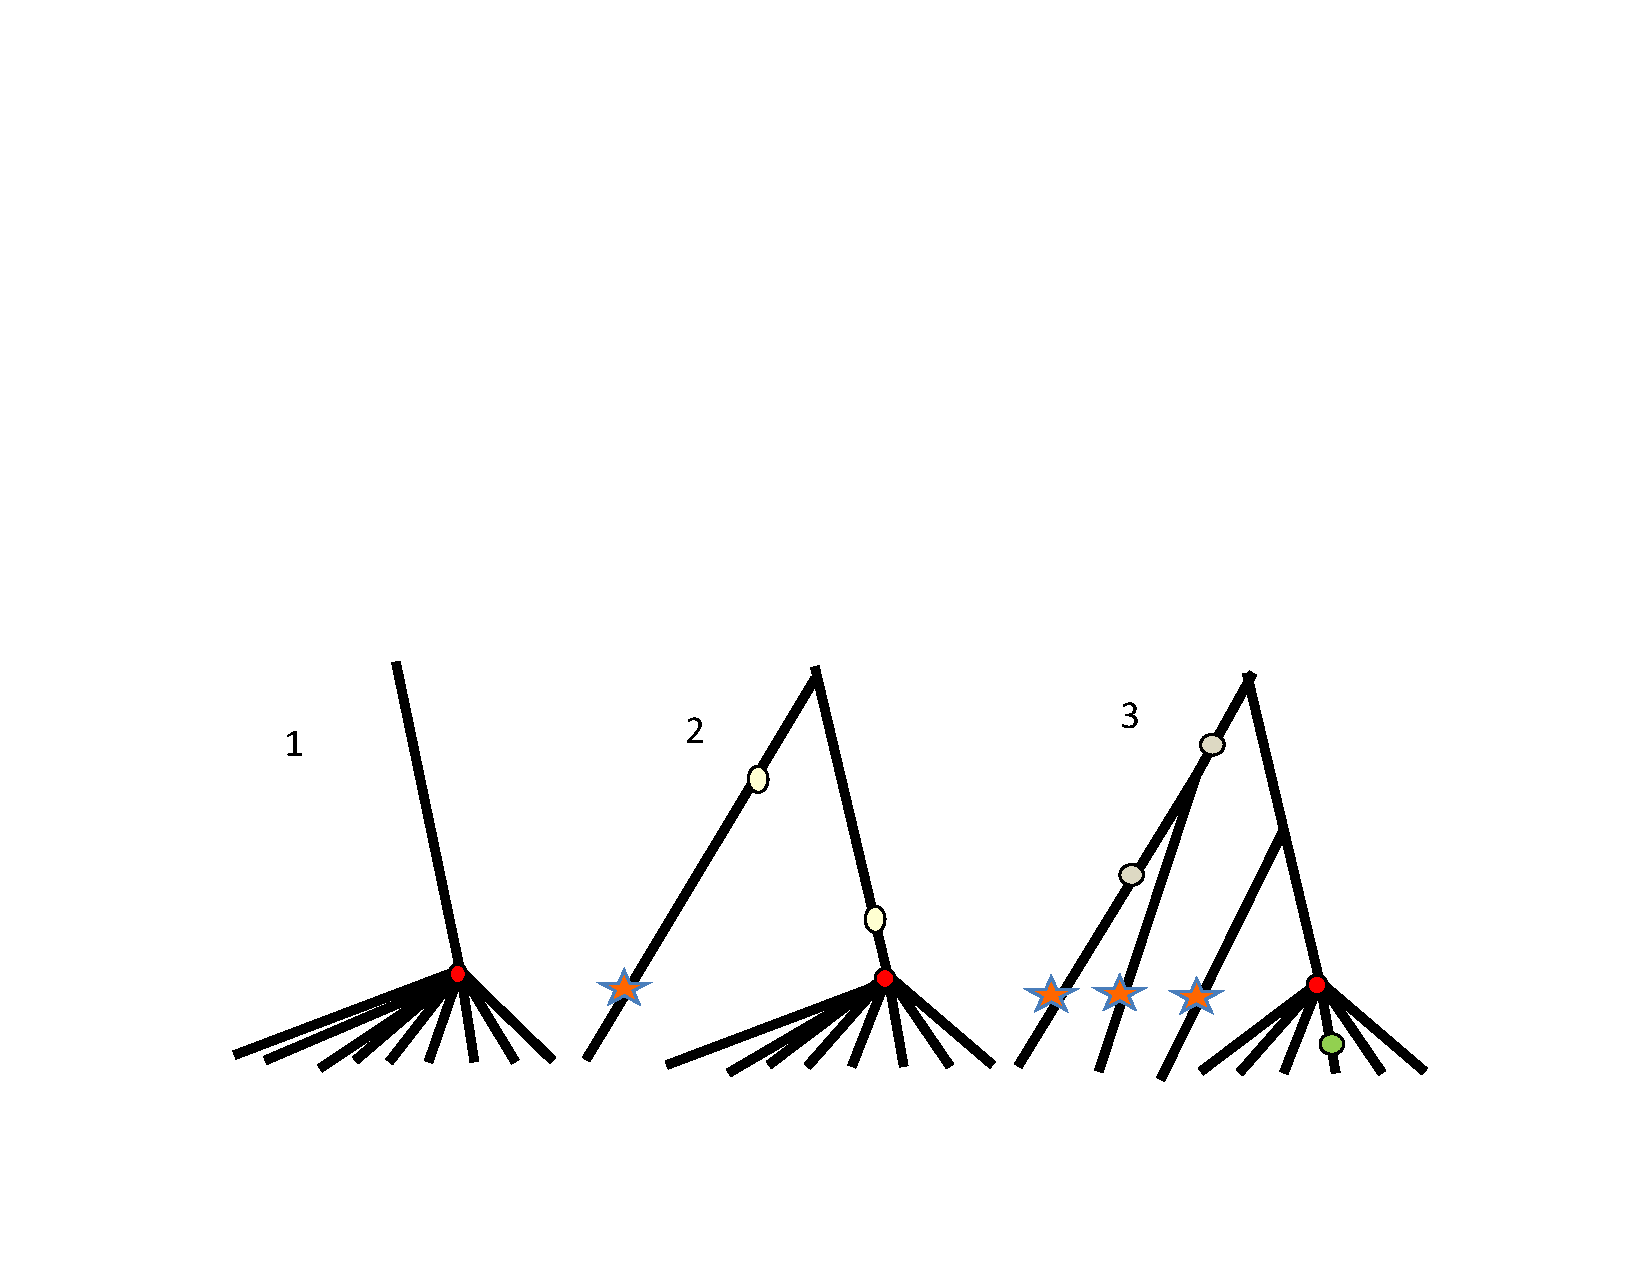
\includegraphics[width= 0.9 \textwidth]{figures/Hitchhiking/recom_haps_coal_sweep.pdf}
\end{center}
\caption{Coalescent genealogies at three loci different distances along the genome from a selective sweep. The locations of these three loci along the genome are marked in Figure \ref{fig:sweep_haps}. The selected mutation is shown in red. Lineages descended from recombination events during the sweep are marked in stars. Neutral mutations close to each of the loci are shown on the genealogy.} \label{fig:sweep_haps_coal}
\end{figure}

What do the coalesecent genealogies look like at loci various distances away from the
selected site? Well, close to the selected site all our alleles in the
present day trace back to a most recent common ancestral allele
present on that selected haplotype, and so are all forced to coalesce
around $\tau$ generations ago (locus 1, see Figure \ref{fig:sweep_haps_coal}). Slightly further out from the selected
site (locus 2), we have lineages that don't trace their ancestry back
to the original selected haplotype, but instead are descended from
recombinant haplotypes that recombined onto the sweep (the haplotype second from the
bottom in Figure \ref{fig:sweep_haps_coal}). These lineages can coalesce neutrally with the other ancestral lineages
over far deeper time scales and mutations on these deeper lineages
correspond to the standing diversity present in our population
prior to the sweep. As we move even further out from the selected site
(locus 3), we encounter more and more lineages descended from
recombinant haplotypes that coalesce neutrally much deeper in time than $\tau$, 
allowing diversity to recover to background levels as we move away
from the selected site (see Figure \ref{fig:hitchhiking_reduction}).

\begin{figure}
\begin{center}
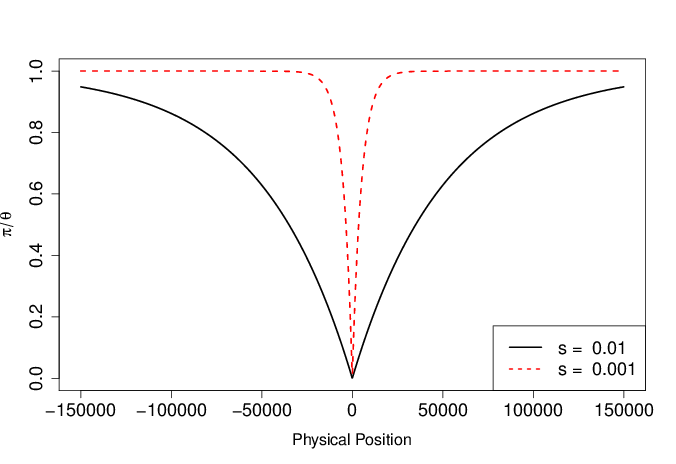
\includegraphics[width=0.75\textwidth]{figures/hitchhiking_reduction.png}
\end{center}
\caption{The expected reduction in diversity compared to its neutral expectation as
a function of the distance away from a site where a selected allele
has just gone to fixation. The sweeps associated with two different strengths of selection are shown, corresponding to a short timescale ($\tau$) for the sweep and long one. The recombination rate is $c_{BP}= 1\times
10^{-8}$. \gitcode{https://github.com/cooplab/popgen-notes/blob/master/Rcode/Hitchhiking.R}} \label{fig:hitchhiking_reduction}
\end{figure}


To model the expected pattern of diversity surrounding a selected site, we can think about a pair
of alleles sampled at a neutral locus a recombination distance $c$
away from our selected site. Our pair of alleles will be forced to
coalesce $\approx \tau$ generations if neither of them of are
descended from recombinant haplotypes (Left side of Figure \ref{fig:recom_coal}).\\
\begin{marginfigure}
\begin{center}
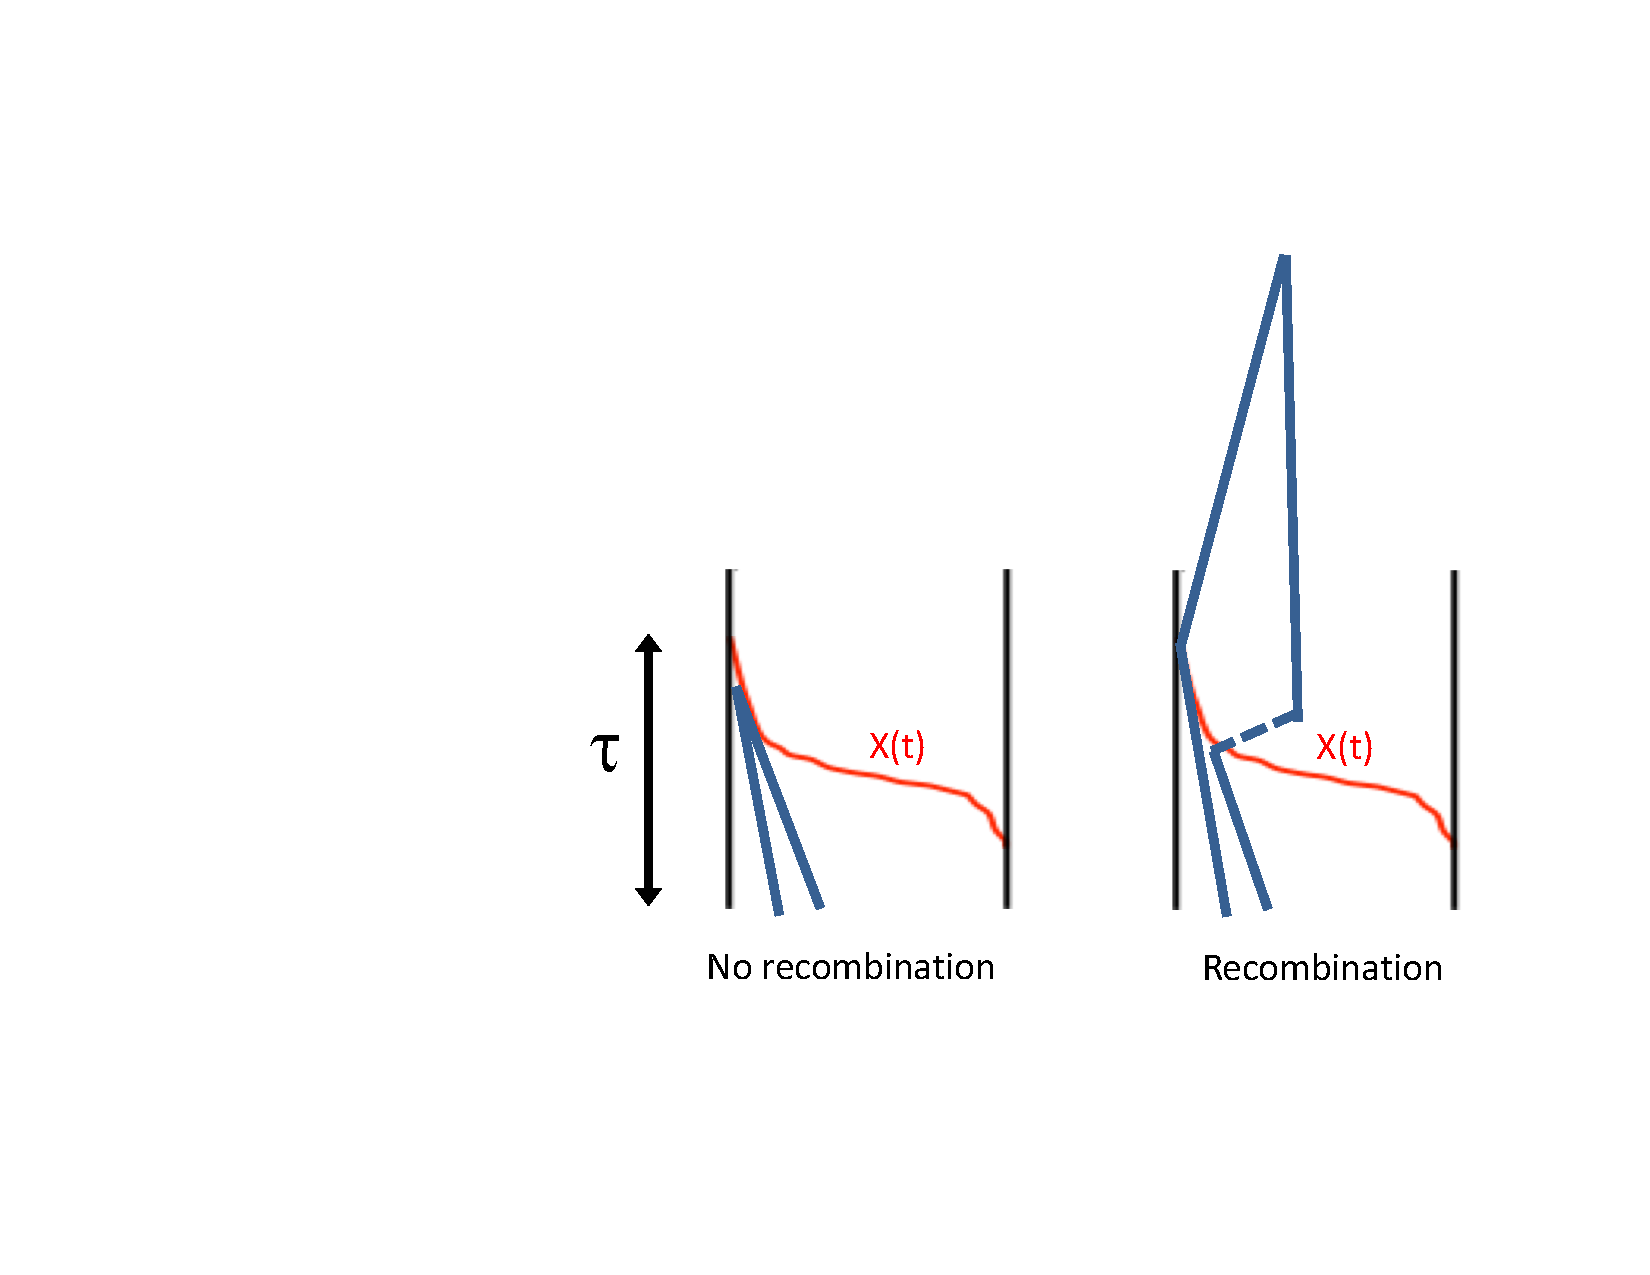
\includegraphics[width= \textwidth]{figures/Hitchhiking/Recom_coal.pdf}
\end{center}
\caption{{\bf Left)} two lineages coalesce roughly $\tau$ generations
  ago as they are both descended from the selected haplotypes. {\bf Right)}
One of our two lineages is descended from the selected haplotype but
the other is descended from a recombinant on to the sweep. The pair on
the right coalesce much deeper back in time.} \label{fig:recom_coal}
\end{marginfigure}
The probability that our alleles at our neutral locus is descended
from the ancestral haplotype on which the selected allele occurs,
i.e. that the alele does not descend from a recombinant haplotype is
\begin{equation}
p_{NR} = e^{-c \tau/2 }. \label{eqn:prob_no_recom_sweep}
\end{equation}
What's the intuition for this werll there are $\tau$ generations in
which a recombination can occur, so roughly the probability that
absolutely no recombination occurs is $(1-c)^{\tau} =\approx
e^{-c\tau}$. Where does the factor of $\nicefrac{1}{2}$ in \eqn
\eqref{eqn:prob_no_recom_sweep} come from? Well in order to recombine an allele off the selected background the
recombination must occur in a heterozygote for the selected allele,
under an additive model a neutral allele linked to a fully sweeping allele
spends on average $\nicefrac{1}{2}$ its time in heterozyotes so
reducing our effective recombination rate by a factor of two (see
Appendix \ref{Appendix:no_recom_sweep} at the end of the chapter for
more details).\\

The probability that neither of our lineages is descended from a
recombinant haplotype, and hence are forced to coalesce, is $p_{NR}^2$ (assuming that
they coalesce at a time close to $\tau$ so that they recombine
independently of each other for times $< \tau$).
If one or other of our lineages is descended from a recombinant haplotype, it will take them on average
$\approx 2N$ generations to find a common ancestor, as we are back to our
neutral coalescent probabilities (Right side of Figure \ref{fig:local_sweep_haps}). Thus, the expected time
till our pair of lineages find a common ancestor is
\begin{equation}
\E(T_2)  = \tau \times p_{NR}^2 +(1-p_{NR}^2) (\tau +2N) \approx
\left(1-p_{NR}^2 \right) 2N
\end{equation}
where this last approximation assumes that $\tau \ll 2N$. So the
expected pairwise diversity for neutral alleles at a recombination
distance $r$ away from the selected sweep ($\pi_c$) is
\begin{equation}
\E(\pi_c) = 2\mu \E(T_2)  \approx \pi_0 \left(1-e^{-c\tau} \right) \label{eqn:pi_HH}
\end{equation}
So diversity increases as we move away from the selected site,
slowly and exponentially plateauing to its neutral expectation
$\pi_0$.\\
\begin{marginfigure}
\begin{center}
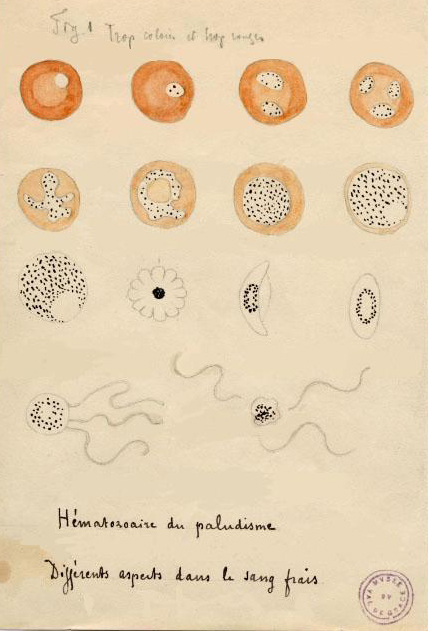
\includegraphics[width=\textwidth]{illustration_images/hitchhiking/malaria/Laveran_Malaria_drawings.jpg}
\end{center}
\caption[][-0.5cm]{Laveran's 1880 drawing of various stages of {\it Plasmodium
    falciparum} as seen in fresh blood. The bottom row shows an
  exflagellating male gametocyte. Laveran identified {\it P. falciparum} as the
  protozoan pathogen that caused malaria. \wikimedia{\href{Centers for
    Disease Control and Prevention (caption modified).}}{https://commons.wikimedia.org/wiki/File:Laveran_Malaria_drawings.jpg}{TimVickers}{ United States public domain}} \label{fig:malaria}
\end{marginfigure}

% \begin{marginfigure}
% \begin{center}
% 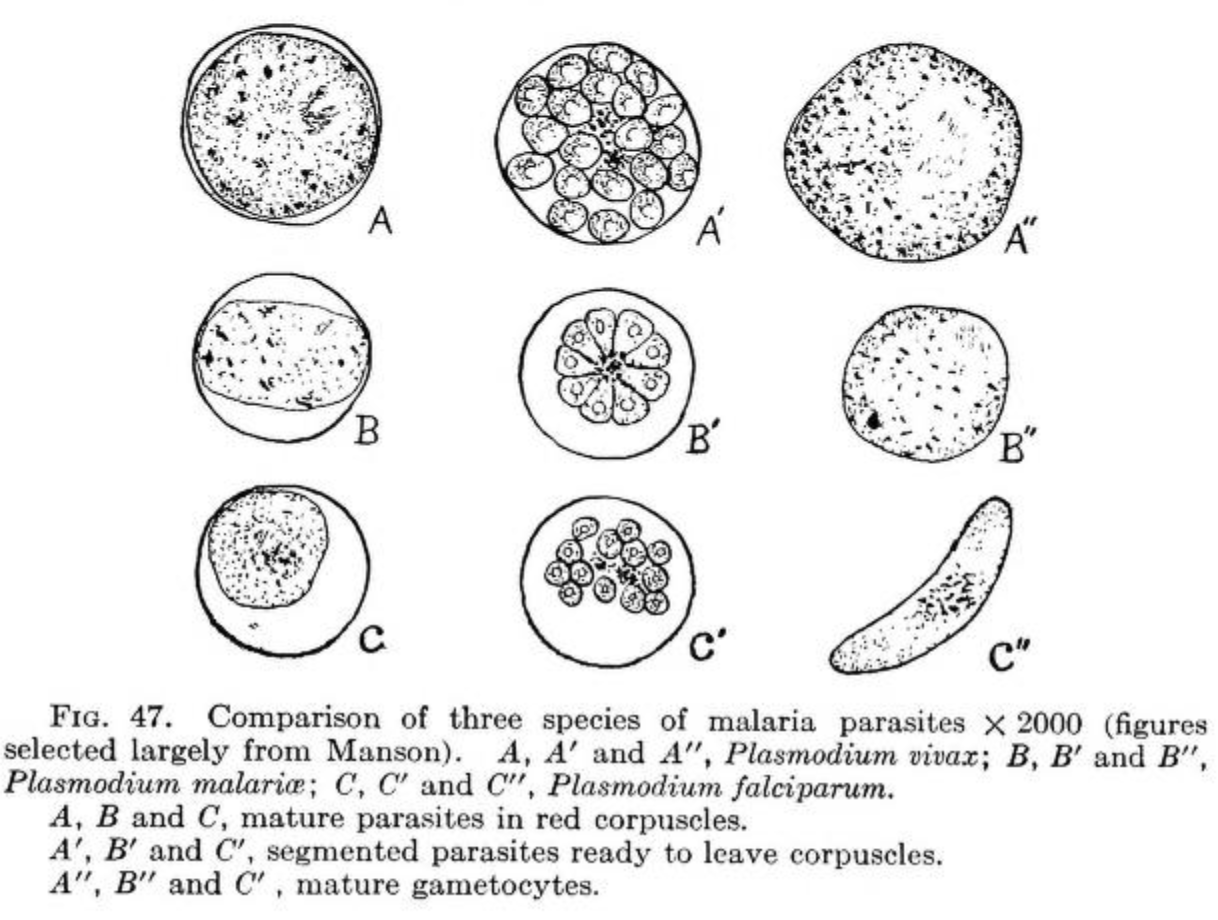
\includegraphics[width=\textwidth]{illustration_images/hitchhiking/malaria/malaria.png}
% \end{center}
% \caption{Three species of malaria parasites ({\it Plasmodium}) in red
%   blood cells. \BHLNC{Animal parasites and human disease (1918). Chandler, A.C.}{https://www.flickr.com/photos/internetarchivebookimages/20181659403/}{Cornell University Library} } \label{fig:malaria}
% \end{marginfigure}
The malaria pathogen ({\it Plasmodium falciparum}) has
evolved drug resistance to anti-malaria drugs, often by changes at
the dhfr gene. Figure \ref{fig:hitchhiking_malaria} shows levels of
genetic diversity (heterozygosity) at a set of markers moving out from the dhfr gene in a
set of  drug resistant malaria sequences collected in
Thailand \citep{nash2005selection}. We see the characteristic dip in diversity around the gene,
with zero diversity at a number of the loci very close to the gene,
suggesting a strong selective sweep. Fitting our simple model of a
sweep to this data,  we estimate that $\tau \approx 40$ generations,
corresponding to the drug-resistance allele fixing in very short time period. 
% these drug (Sulfadoxine–pyrimethamine) 

\begin{figure}
\begin{center}
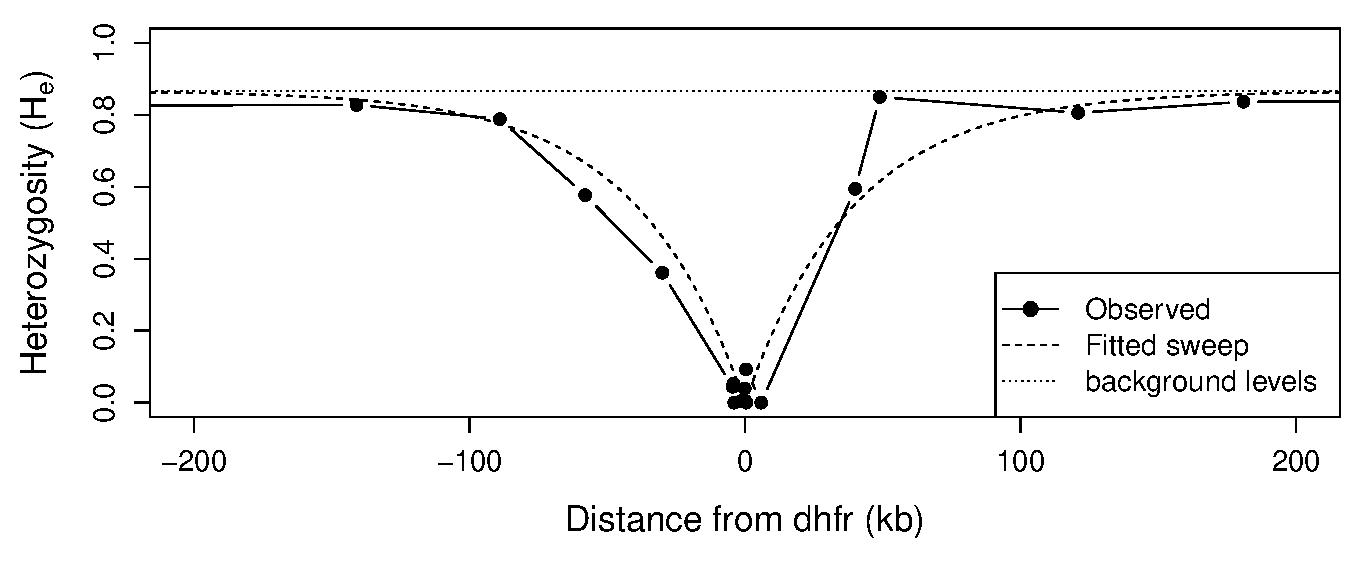
\includegraphics[width=\textwidth]{Journal_figs/recom_selection/malaria_sweep/dhfr_sweep.pdf}
\end{center}
\caption[][5cm]{Levels of heterozygosity at a set of microsatellite markers
  surounding the dhfr gene in samples of drug-resistant malaria ({\it Plasmodium falciparum}) from
  Thailand. The dotted horizontal line gives the average level of
  heterozygosity found at these markers in a set of drug-resistant
  malaria; we take this background as our $\pi_0$. The dashed line shows
  our fitted hitchhiking model from equation \ref{eqn:pi_HH} with $\tau \approx 40$, fitted by
  non-linear least squares. The recombination rate in {\it P.
    falciparum} is $c_{BP}\approx 10^{-6}$bp$^{-1}$. Data from
  \citet{nash2005selection}. \gitcode{https://github.com/cooplab/popgen-notes/blob/master/Journal_figs/recom_selection/malaria_sweep/dhfr_sweep.R}} \label{fig:hitchhiking_malaria}
\end{figure}


To get a sense of the physical scale over which diversity is reduced,
consider a region where recombination occurs at a rate $c_{BP}$ per
base pair per generation, and a locus $ \ell $ base pairs away from the
selected site, such that $c=c_{BP } \ell $ (where $c_{BP}  \ell  \ll 1$ so we don't need to
worry about more than one recombination event occurring per
generation). Typical
recombination rates are on the order of $c_{BP} = 10^{-8}$. In Figure
\ref{fig:hitchhiking_reduction} we show the reduction in diversity,
given by eqn. \eqref{eqn:pi_HH}, for two different selection coefficients.\\ 

For our expected diversity level to recover to $50\%$ of
its neutral expectation $\E(\pi_c)/\theta=0.5$, requires a physical
distance $\ell^{*}$ such that $\log(0.5) = -x_{BP} \ell ^*\tau$, and by re-arrangement,
\begin{equation}
\ell^* = \frac{-\log(0.5)}{c_{BP} \tau }.
\end{equation}
As
$\tau$ depends inversely on the selection $s$ (eqn. \eqref{eq:diploid_fix_time}), the width of our trough of reduced diversity depends on $s/c_{BP}$.
All else being equal, we expect stronger sweeps or sweeps in regions of low
recombination to have a larger hitchhiking effect. For example, in a genomic region with a recombination rate $c_{BP}=10^{-8}$bp$^{-1}$ a selection coefficient of $s=0.1\%$ would reduce
diversity over 10's of kb, while a sweep of $s=1\%$ would affect
$\sim$100kb.   \\



\begin{question}{}
\citet{van2011industrial}  identified the genetic basis of
melanism in the peppered moth ({\it Biston betularia}). This allele swept to fixation in northern
parts of the UK; a classic case of adaptation to industrial pollution
(made famous by the work of \citeauthor{kettlewell1955selection}, see
\citet{majerus2009industrial} and \citet{cook2012selective}). The genetic basis of melanism
is a transposable element (TE) inserted into a pigmentation gene. \citeauthor{van2011industrial} found that diversity is suppressed in a broad region
around the TE. Specifically, on the background of the TE, it takes
roughly 200 kb in either direction for diversity levels to recover to
50\% of genome-wide levels. \\

Random facts: In all moths and butterflies only males recombine;
chromosomes are transmitted without recombination in females. The
recombination rate in males is 2.9 cM/Mb.  Peppered moths have an
effective population size of roughly a hundred thousand
individuals. Kettlewell used to eat moths when out collecting them in
the field (personal communication, Art. Shapiro). \\
{\bf A)} Briefly explain how this pattern offers further evidence that the melanic allele was favoured by selection.\\
{\bf B)} Using this information, and assuming the allele's effects on fitness are additive, what is your estimate of the age of the allele? \\
{\bf C)} What is your estimate of the selection coefficient favouring this melanic allele?
\end{question}
\begin{marginfigure}[-3cm]
\begin{center}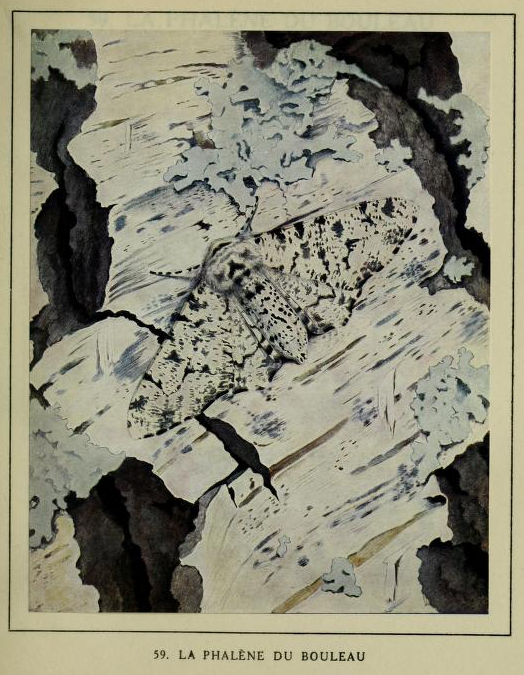
\includegraphics[width= \textwidth]{illustration_images/hitchhiking/Pepper_moth/lespapillonsdans01robe_0375_trimmed.png}
\end{center}
\caption{Peppered moth ({\it Biston betularia}), non-melanic morph \BHLNC{Les papillons
    dans la nature (1934).Robert, P.-A. }{https://www.biodiversitylibrary.org/page/33080243\#page/367/mode/1up}{University of Illinois Urbana-Champaign} } \label{Peppered_moth}
\end{marginfigure}

\paragraph{Other signals of selective sweeps}
The primary signal of a recently completed selective sweep is the
characteristic reduction in diversity surrounding the selected site.
However, sweeps do leave other signals, and these have also often been
used to identify loci undergoing selection. 
For example, neutral alleles further away from the selected site may
hitchhiw only part of the way to fixation if recombination occurs during
the sweep, which can lead to an excess of high-frequency
derived alleles at intermediate distances away from the selected site,
a pattern lasting for a short time after a sweep \citep{Fay:00,Przeworski:02,Kim:06}.
Also, as neutral diversity levels slowly recover through an influx of
new mutations after a sweep, there is a strong skew towards low
frequency derived alleles, a pattern that persists for many
generations \citep{Braverman:95, Przeworski:02,Kim:06}. The excess of
rare alleles, compared to a neutral model, can be captured by
statistics such as Tajima's {\it D} (which
we encountered back in our discussion of the neutral site frequency eqn
\ref{eqn_Tajimas_D}). Thus one way to look for loci that have
undergone selective sweeps is to calculate Tajima's {\it D} from data in
windows along the genome and look for
strong departures from the null distribution.

\begin{figure}
\begin{center}
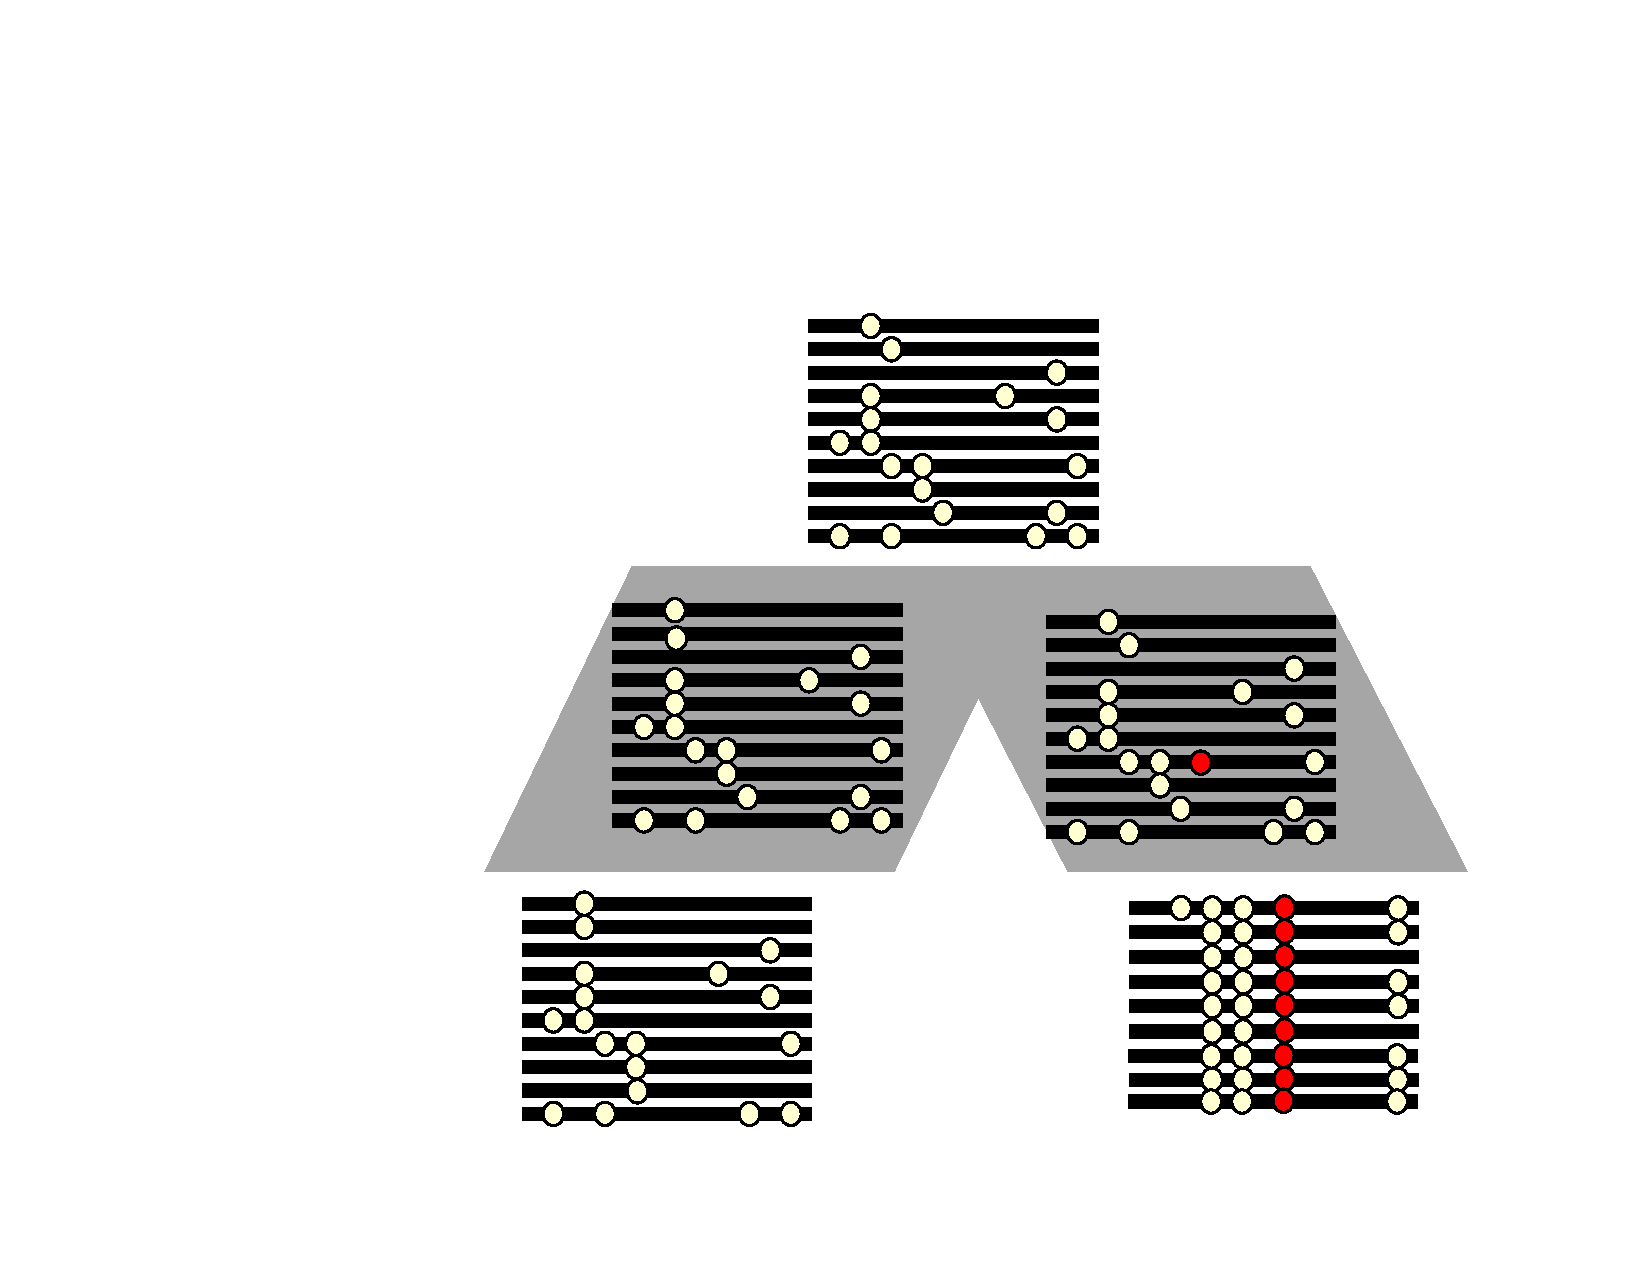
\includegraphics[width=0.5 \textwidth]{figures/Hitchhiking/two_pops_sweep.pdf}
\end{center}
\caption{Two populations descended from a common ancestral
  population. A beneficial mutation has occurred in population and
  swept to fixation.} \label{fig:local_sweep_haps}
\end{figure}

We can also use comparisons among multiple populations to look for evidence of sweeps occurring in one of the
populations, for example to identify alleles involved in local adaptation (see \ref{fig:local_sweep_haps}). A selective sweep will decrease the within-population diversity ($H_S$)
surrounding the selected site, without affecting the diversity between different
populations. Thus local sweeps create peaks of
$\fst$ between weakly differentiated populations. 

\citet{hohenlohe2010population} studied genome-wide patterns of
$\fst$ between marine and freshwater populations of  threespine
stickleback ({\it Gasterosteus aculeatus}), plotted in Figure \ref{fig:local_sweep_stickleback}. 
Between different marine populations, they found no strong peaks of $\fst$;
however, between the marine and freshwater comparisons they found a
number of high $\fst$  peaks that were replicated over a number of
freshwater-marine comparisons. They identified a number of novel
regions responsible for the adaptation of sticklebacks to freshwater
environments and also a number of loci previously identified in crosses between marine and freshwater populations. For example, the first peak of Linkage
Group IV includes {\it Ectodysplasin A} ({\it Eda}), a gene involved in the adaptive loss of armour plating in freshwater environments.
\begin{figure}
\begin{center}
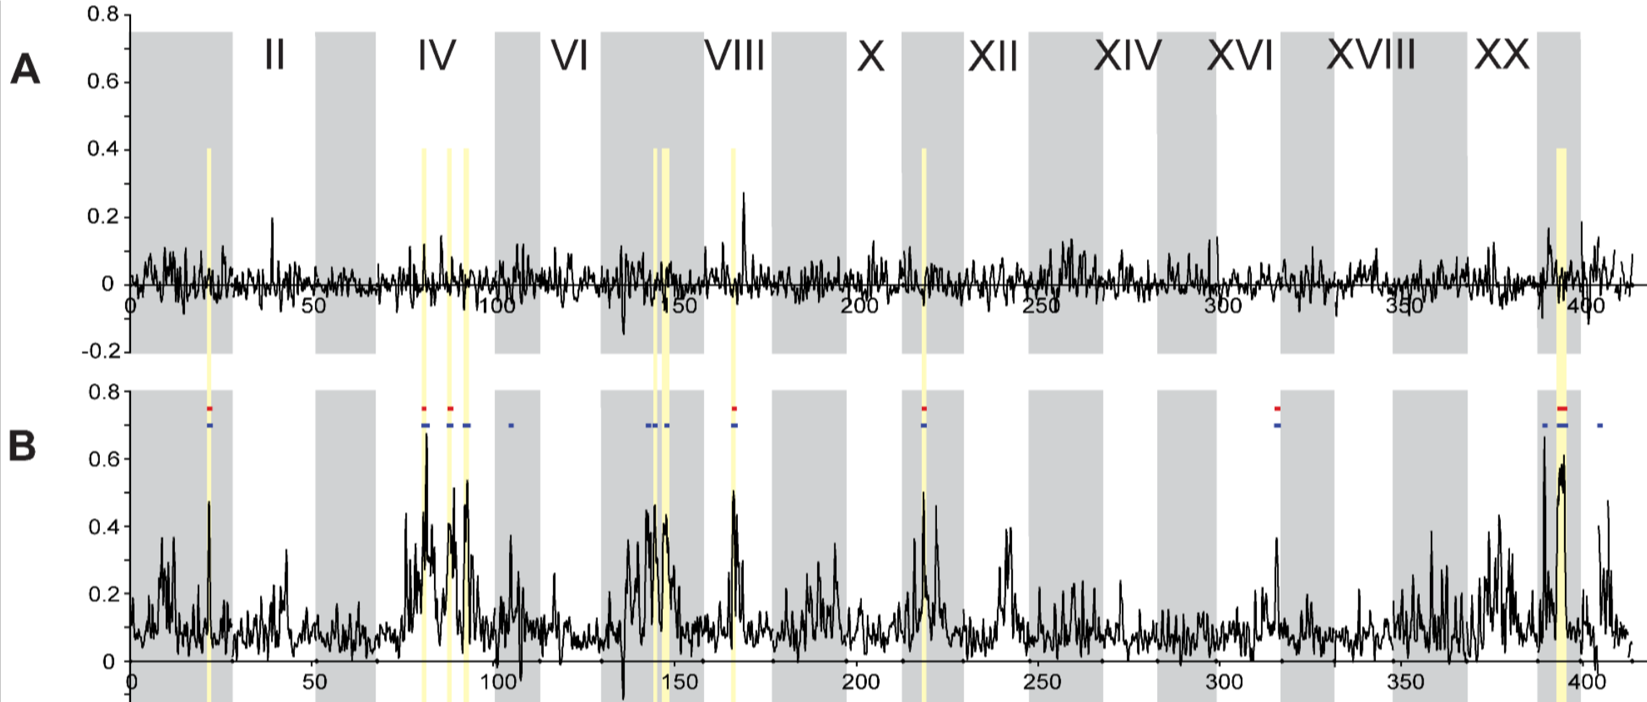
\includegraphics[width=0.9 \textwidth]{Journal_figs/recom_selection/Stickleback_FST/hohenlohe.png}
\end{center}
\caption{$\fst$ across the stickleback genome, with colored bars indicating
  significantly elevated ($p \leq 10^{−5}$, blue; $p \leq 10^{−7}$,
  red) and reduced ($p \leq 10^{−5}$, green) values. The alternating
  white and grey panels indicate different linkage groups. {\bf A)} $\fst$
  between two oceanic populations {\bf B)} Average $\fst$ between a
  freshwater population and the two marine populations. Figure and
  caption text from \citet{hohenlohe2010population}, \PLOSccBY.} \label{fig:local_sweep_stickleback}
\end{figure}


\paragraph{Soft Sweeps from multiple mutations and standing variation.}
In our sweep model above, we assumed that selection favoured a
beneficial allele from the moment it entered the population as a
single copy mutation  (left panel, Figure \ref{fig:soft_sweep_haps}). However, when a novel selection pressure
switches on, multiple mutations at the same gene
may start to sweep, such that no one of these alleles sweeps
to fixation (middle panel, Figure \ref{fig:soft_sweep_haps}). These sweeps involving multiple mutations significantly
soften the impact of selection on genomic diversity, and so are called 'soft sweeps'.

\begin{figure}
\begin{center}
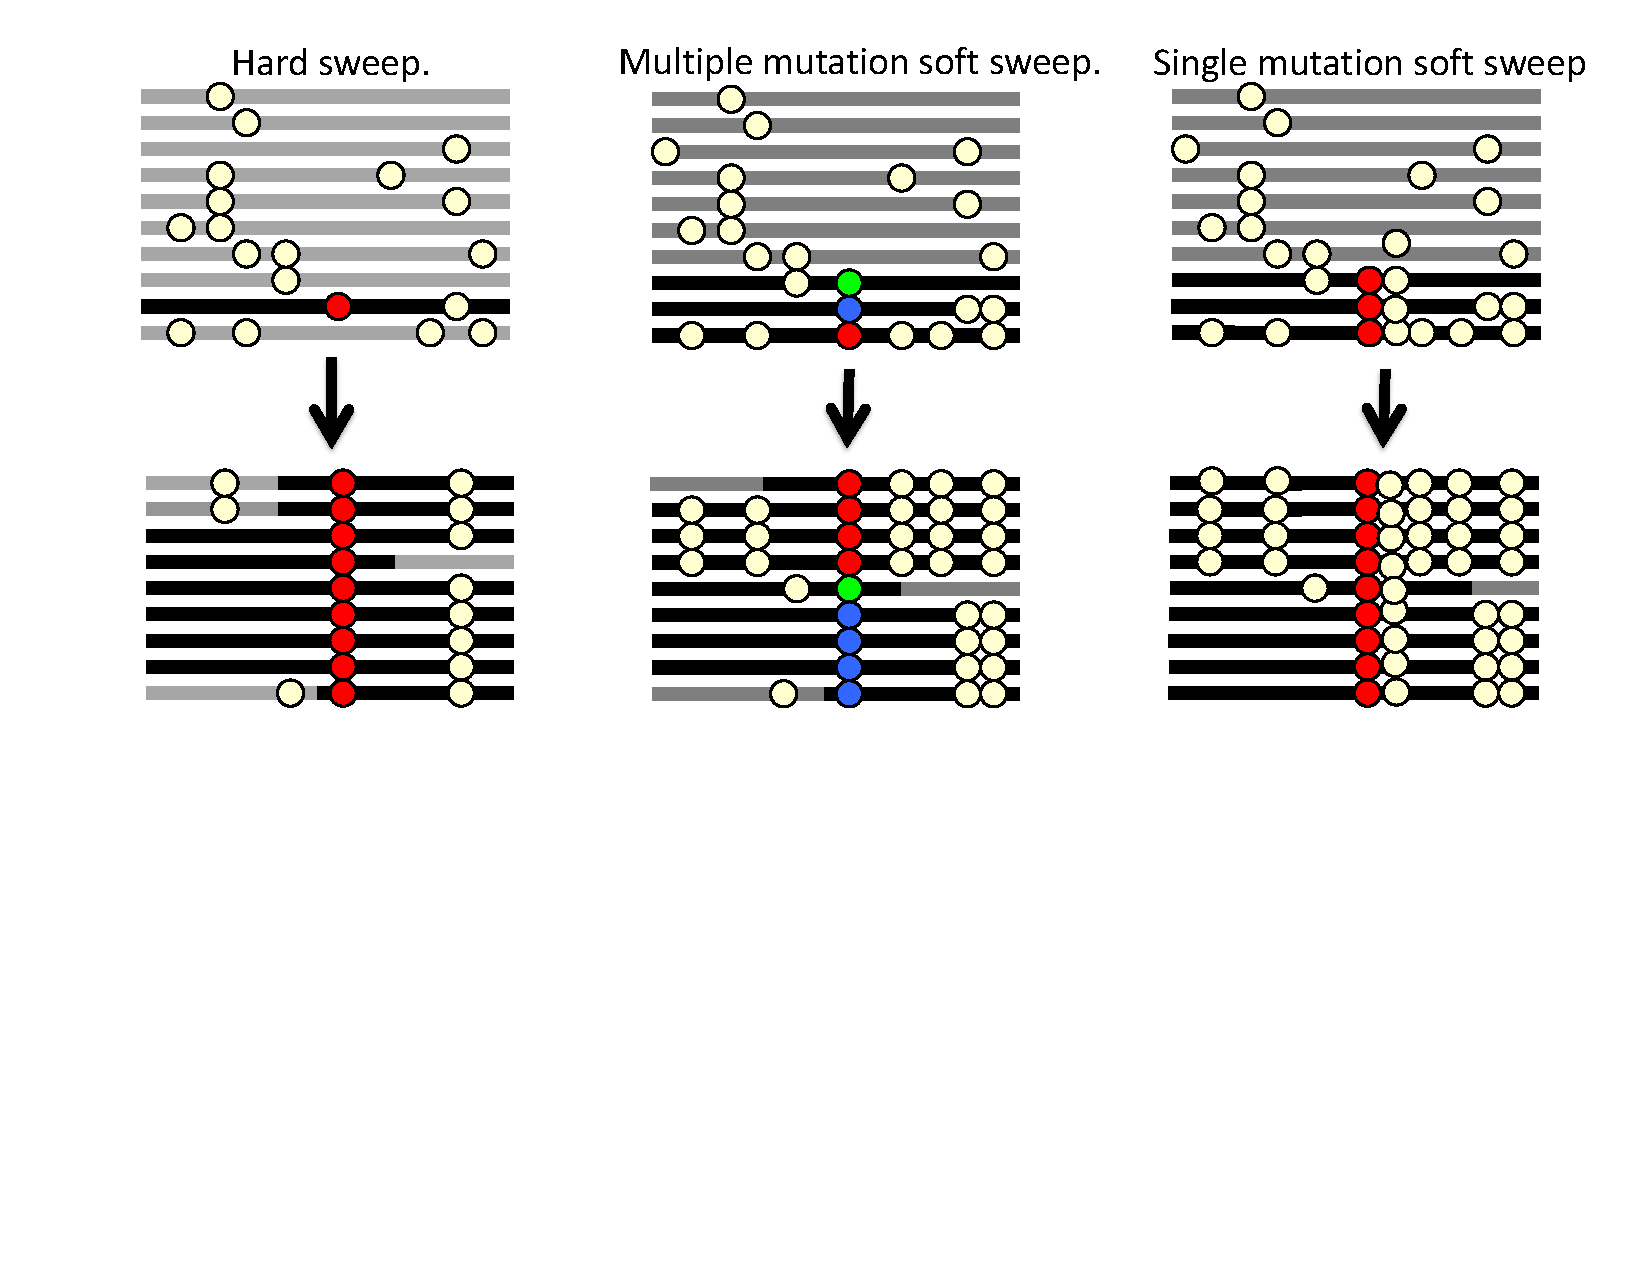
\includegraphics[width=\textwidth]{figures/Hitchhiking/Soft_sweeps.pdf}
\end{center}
\caption{Three types of sweeps. } \label{fig:soft_sweep_haps}
\end{figure}

Another way that the impact of a sweep can be softened is if our
allele was segregating in the population for some time before it
became beneficial. That additional time means that our allele can have
recombined onto various haplotype backgrounds, such that when
selection pressures switch, the selected allele sweeps up in frequency on 
multiple different haplotypes (right panel, Figure \ref{fig:soft_sweep_haps}). 
Detecting and differentiating these different types of sweeps is an active area of
empirical research and theory in population genomics (see \citet{hermisson2017soft} for an overview of
developments in this area).

%For example recall the multiple mutations at G6PD
%in the prior chapter. 

\section{The genome-wide effects of linked selection.}
To what extent are patterns of variation along the genome and
  among species shaped by linked selection, such as selective sweeps? 
We can hope to identify individual cases of strong selective sweeps
along the genome, but how do they contribute to broader patterns of
variation?

 Two observations have puzzled population geneticists since the
inception of molecular population genetics. The first is the relatively high
level of genetic variation observed in most obligately sexual species.  
The neutral theory of molecular evolution was developed in part to
explain these high levels of diversity. As we saw in Chapter \ref{Chapter:Drift}, 
under a simple neutral model, with constant population size, we should expect the amount of neutral genetic
diversity to scale with the product of the population size and
mutation rate. The second observation, however, is the relatively narrow range 
of polymorphism across species with vastly different census sizes (see
Figure \ref{fig:Leffer} and \citet{leffler:12} for a recent review). 
As highlighted by \citet{Lewontin:74} in his discussion of the paradox
of variation, this observation seemingly contradicts the prediction of the neutral theory that
genetic diversity should scale with the census population size. There are a number of explanations for the discrepancy between genetic
diversity levels and census population sizes. The first is that the effective size of the population ($N_e$) is
often much lower than the census size, due to high variance in
reproductive success and frequent bottlenecks (as discussed in  Chapter \ref{Chapter:Drift}). 
The second major explanation, put forward by \citet{MaynardSmithHaigh74},
is that neutral levels of diversity are also systematically reduced by the effects of linked selection. 
In large populations, selective sweeps and other forms of linked selection may come to dominate over genetic drift as a
source of stochasticity in allele frequencies, potentially establishing an upper limit to levels of diversity \citep{Kaplan:89, Gillespie:00}. 

\begin{figure}
\begin{center}
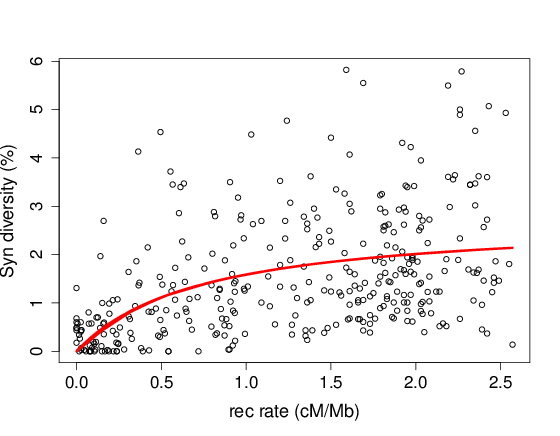
\includegraphics[width=0.75\textwidth]{figures/Genomewide_HH.png}
\end{center}
\caption{The relationship between (sex-averaged) recombination rate and synonymous
  site pairwise diversity ($\pi$) in {\it Drosophila melanogaster}. The curve is the
  predicted relationship between $\pi$ and recombination rate, obtained
  by fitting the recurrent hitchhiking equation \eqref{eqn:pi_GW_HH} to this data 
 using non-linear least squares via the {\tt nls()} function in {\tt
   R}.  Data from \citep{Shapiro:07}, kindly provided by Peter
  Andolfatto, see \citet{sella2009pervasive} for details. \gitcode{https://github.com/cooplab/popgen-notes/blob/master/Rcode/Genomewide_HH.R}} \label{fig:GW_hitchhiking_reduction}  %%Code source('~/Dropbox/Courses/Popgen_teaching_Notes/Rcode/Genomewide_HH.R')
\end{figure}

%Hellmann:08,, cutter2013
One strong line of evidence for the action of linked selection in reducing levels of
polymorphism is the positive correlation between putatively
neutral diversity and recombination seen in a number of species, as, all
else being equal, linked selection should remove diversity more quickly in regions of low recombination 
\citep{Aguade:89,Begun:92,Wiehe:93,Cutter:10,Cai:09}. For example, {\it Drosophila melanogaster} diversity
levels are much lower in genomic regions of low recombination (see
Figure \ref{fig:GW_hitchhiking_reduction}). This pattern can not be
explained by differences in mutation rate between low and high
recombination regions as this pattern is not seen strongly in
divergence data among species.

These patterns could reflect the action of selective sweeps happening
recurrently along the genome. In the next section we'll present a model for how levels of
genetic diversity should depend on recombination and the density of
functional sites under a model of recurrent selective sweeps.
However, other forms of linked selection can impact genetic
diversity in similar ways. For example, linked genetic diversity is
continuously lost from natural populations due to the removal of
haplotypes that carry deleterious alleles
\citep{Charlesworth:95,Hudson:95}; this is called the 'background selection'
model. Below we'll discuss the background selection model and its
basic predictions.

%,Neher:13,Good:14
More generally, a wide range of models of selection predict the removal of neutral
diversity linked to selected sites. This is because the diversity-reducing effects of high variance in reproductive success are compounded over the generations when there is heritable variance in fitness 
\citep{Robertson:61,Santiago:95,Santiago:98,Barton:00}.  Many
different modes of linked selection likely contribute to these
genome-wide patterns of diversity; the present challenge is how to
differentiate among these different modes.


\subsection{A simple recurrent model of selective sweeps}
To explain how a constant influx of sweeps could impact levels of
diversity, here we will develop a model of recurrent
selective sweeps.

Imagine we sample a a pair of neutral alleles at a locus a genetic distance $c$ away from a locus where
sweeps are initiated within the population at some very low rate $\nu$
per generation. The waiting time between sweeps
at our locus is exponentially distributed $\sim Exp(\nu)$ (see math
Appendix \eqn \eqref{eqn:exp_rv_def}). Each sweep rapidly transits through the population in $\tau$
generations, such that each sweep is finished long before the next
sweep ($\tau \ll \nicefrac{1}{\nu}$). \\

As before, the chance that our neutral lineage fails to recombine
off the sweep is $p_{NR}$, such that the probability that
our pair of lineages are forced to coalesce by a sweep is $e^{-c \tau}$. Our
lineages therefore have a very low probability
\begin{equation}
\nu e^{-c \tau}
\end{equation}
of being forced to coalesce by a sweep per generation. If our lineages do not coalesce due to a sweep, they coalesce at a neutral rate of $\nicefrac{1}{2N}$ per generation. Thus the average
waiting time till a coalescent event between our neutral pair of
lineages due to either a sweep or a neutral coalescent event is
\begin{equation}
\E(T_2) = \frac{1}{\nu e^{-c \tau} + \nicefrac{1}{2N}}
\end{equation}

Now imagine that the sweeps don't occur at a fixed location with
respect to our locus of interest, but now occur uniformly at random
across our genome. The sweeps are initiated at a very low rate of
$\nu_{BP}$ per basepair per generation. The rate of coalescence due to
sweeps at a locus $\ell$ basepairs away from our neutral loci is
$2\nu_{BP} e^{-c_{BP} \ell \tau}$, where the factor of two comes from
the fact that bases can be $\ell$ basepairs away on the left or right. If our neutral locus is in the
middle of a chromosome that stretches $L$ basepairs in either direction,
the total rate of sweeps per generation that could force our pair of lineages to coalesce is
\begin{equation}
2\int_0^{L} \nu_{BP} e^{-c_{BP} \ell \tau} d \ell =
\frac{2\nu_{BP}}{c_{BP} \tau} \left(1-e^{-c_{BP} \tau L} \right)
\end{equation}
so that if $L$ is very large ($c_{BP} \tau L \gg 1$), the rate of coalescence per
generation due to sweeps is $\nicefrac{2\nu_{BP}}{c_{BP} \tau}$. The total rate
of coalescence for a pair of lineages per generation is then
\begin{equation}
\frac{2\nu_{BP}}{c_{BP} \tau}+\frac{1}{2N}
\end{equation}
So our average time untill a pair of lineages coalesce is
\begin{equation}
\E(T_2) = \frac{1}{\nicefrac{2\nu_{BP}}{c_{BP} \tau}+\nicefrac{1}{2N}} = \frac{c_{BP}2N}{\nicefrac{4N\nu_{BP}}{ \tau}+c_{BP}}
\end{equation}
such that our expected pairwise diversity ($\pi=2\mu\E(T_2)$) in a region with
recombination rate $r_{BP}$ that experiences sweeps at rate $\nu_{BP}$
is  
\begin{equation}
\E(\pi) = \pi_0 \frac{c_{BP}}{\nicefrac{4N\nu_{BP}}{ \tau}+c_{BP}} \label{eqn:pi_GW_HH}
\end{equation}
where $\pi_0$ is our expected diversity without any selective sweeps, ($pi_0=\theta=4N\mu$).  The expected diversity increases with $c_{BP}$, as higher
recombination rates decrease the likelihood a neutral allele hitchhikes along with a sweep and is thus forced to
coalesce by the sweep. Expected diversity decreases with $\nu_{BP}$, as
a greater density of functional sites experiencing sweeps increases the chance of
being linked to a nearby sweep. As we move to high $c_{BP}$, assuming
that $\nu_{BP}$ doesn't increase with $c_{BP}$, our level of diversity
should plateau to $\theta$, the level of genetic diversity of a
neutral site completely unlinked to any selected loci. If we assume
that our genome experiences a constant rate of sweeps of a given
strength, i.e. that $\nicefrac{4N\nu_{BP}}{ \tau}$ is a constant, we can fit the
variation in $\pi$ across regions that vary in their recombination
rate ($c_{BP}$) to estimate a population's rate of recurrent sweeps per basepair.  An example of fitting this curve to data from
{\it Drosophila melanogaster} is shown in Figure
\ref{fig:GW_hitchhiking_reduction}; see \citet{wiehe1993analysis} for
an early example of fitting a similar recurrent hitchhiking model to such data. The parameter giving us this
best-fitting curve is $\nicefrac{4N\nu_{BP}}{ \tau} \approx 7 \times 10^{-9}$. With an
  effective population size of a million  and assuming that the sweeps take
  a thousand generations to reach fixation, we find this implies
  $\nu_{BP} \approx 10^{-12}$. Thus, a really low rate of
  moderately strong sweeps, roughly one every megabase every million
  generations, is all we need to explain the profound dip in diversity seen in regions
  of the genome with low recombination. However, sweeps from positively selected
  alleles are not the only cause of genome-wide signals of linked
  selection. Selection against deleterious alleles can also drive these
  patterns.    
%Assuming that the density of functional sites experiencing sweeps ($\nu+{BP}$) remains the same across recombination environments, i.e. that $r_{BP}$ and $\nu_{BP}$ are uncorrelated 

\subsection{Background selection}

% \citep{sella2009pervasive}
Populations experience a constant influx of
deleterious mutations at functional loci while selection acts to purge
them from the population, thus preventing deleterious substitutions and maintaining function at these loci. As
we discussed in Chapter \ref{Chapter:OneLocusSelection}, this balance between mutation and selection results
in a constant level of deleterious variation in the population. The
constant selection against this deleterious variation has effects on diversity at linked
sites. Each deleterious mutation arises at random on a haplotype in the
population, and as selection purges this mutation, it removes with it any neutral alleles that were also on this
haplotype. This constant removal of linked alleles from the population
acts to reduce diversity in regions surrounding functional loci
\citep{Hudson:95b,Nordborg:96}, an effect known as background
selection (BGS).

What proportion of our haplotypes are free of
deleterious mutations in any given generation, and so free to
contribute to future generations? Well, under mutation-selection
balance, a constrained locus with a mutation rate $\mu$ towards
deleterious alleles that experience a selection coefficient $sh$
against them in heterozygotes, will result in $\nicefrac{\mu}{sh}$
chromosomes carrying the deleterious allele. Some of these haplotypes may be passed on to the next generation, but if they are fully linked to the deleterious locus they will all eventually be lost because they carry a deleterious mutation at a site under constraint. Thus, for a neutral polymorphism
completed linked to a constrained locus, only
$2N(1-\nicefrac{\mu}{sh})$ alleles get to contribute to future
generations. Therefore, the level of pairwise diversity in a constant
population due to BGS at such a locus will be
\begin{equation}
\E[\pi] = 2 \mu \times 2N(1-\nicefrac{\mu}{sh}) = \pi_0  (1-\nicefrac{\mu}{sh})
\end{equation}
where $\pi_0= 4N\mu$, the level of neutral pairwise diversity in the
absence of linked selection.

\begin{figure}
\begin{center}
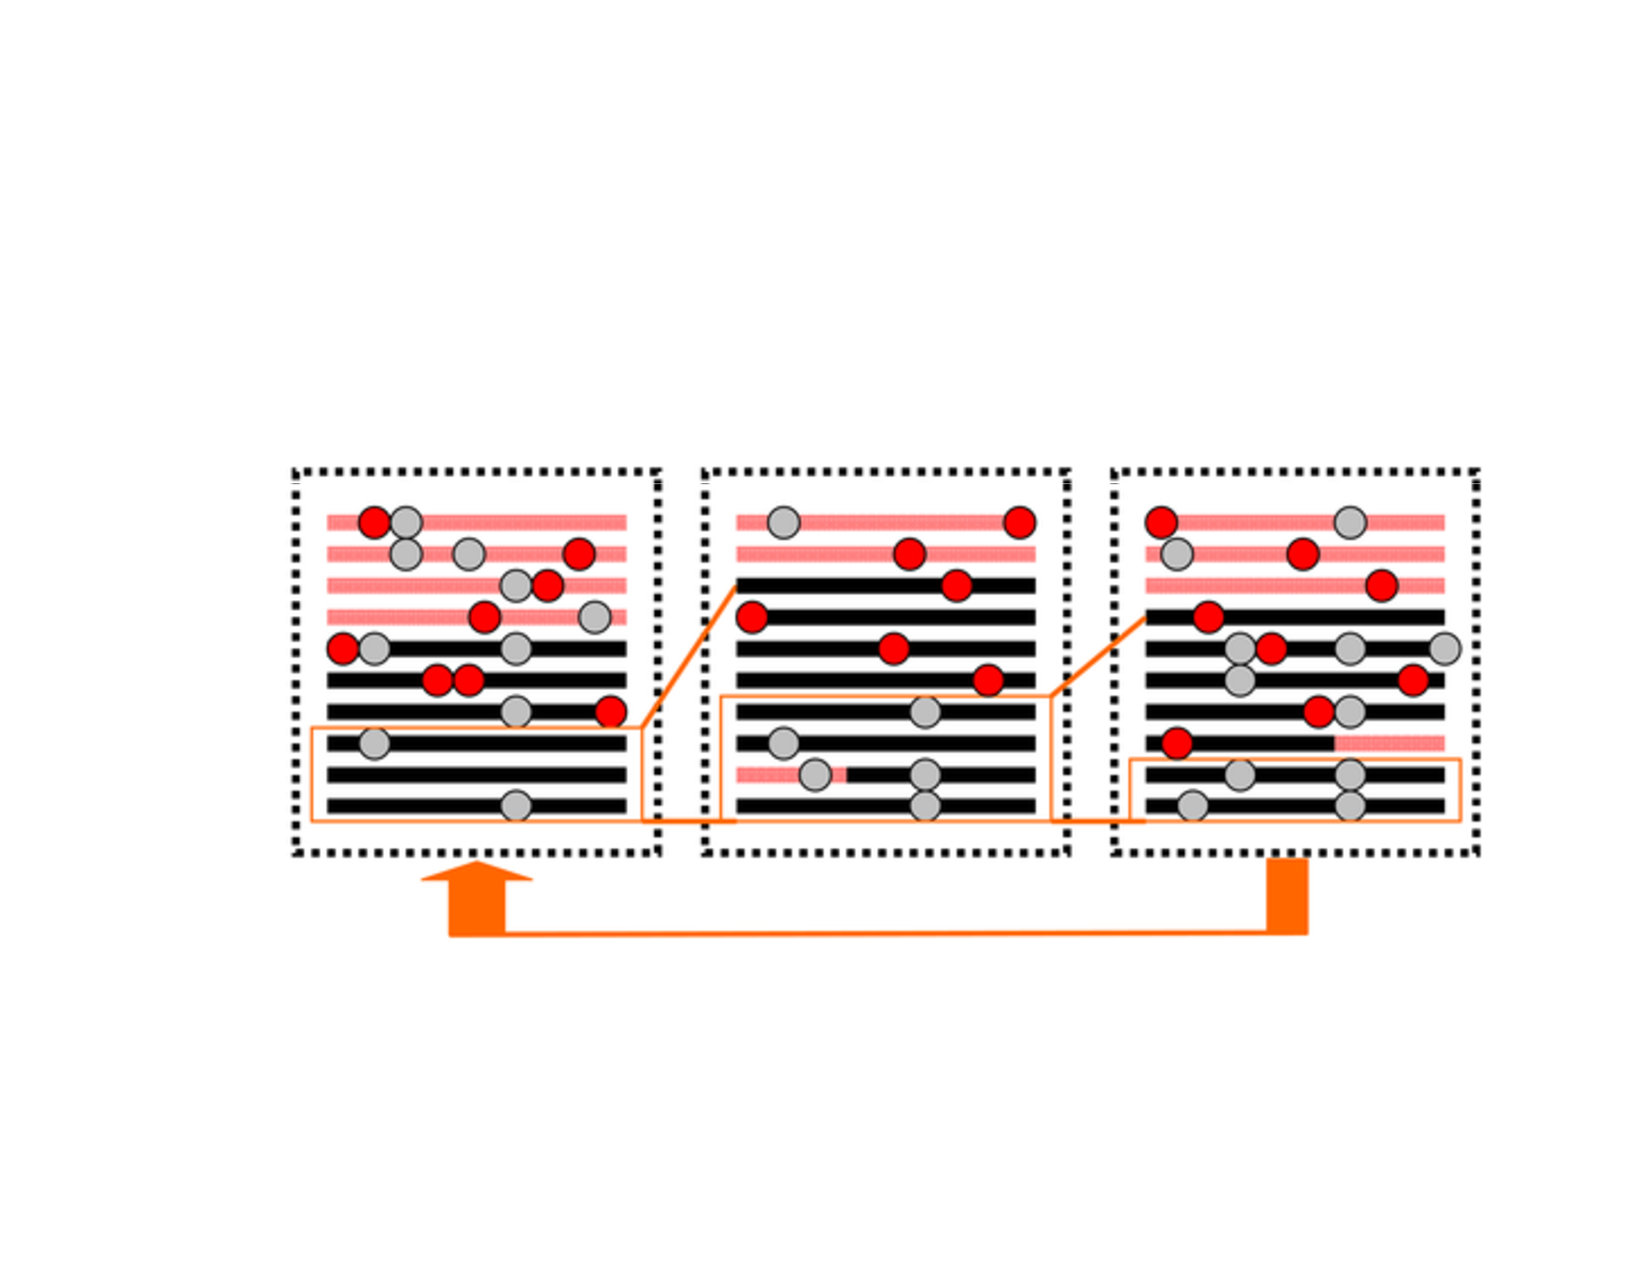
\includegraphics[width=0.75 \textwidth]{figures/Hitchhiking/BGS_cartoon.pdf}
\end{center}
\caption{A cartoon depiction of a region for 10 haplotypes
  experiencing background selection. Neutral mutations are shown as
  gray circles, and deleterious mutations in red. Over time,
  chromosomes carrying deleterious mutations are removed from the
  population, such that most individuals are descended from a subset of
  chromosomes free of deleterious alleles (highlighted here by orange boxes). Mutation is constantly generating new deleterious alleles on
  the background of chromosomes previously free of deleterious
  alleles, and so this process is constantly repeating (orange arrow). Figure modified from \citet{sella2009pervasive}, \PLOSccBY.} \label{fig:BGS_cartoon}
\end{figure}
The effects of background selection are more pronounced in regions of low recombination, where
neutral alleles are less able to recombine off the background of deleterious
alleles. Thus, under background selection, we also expect to see
reduced diversity in regions of lower recombination. 

For a neutral locus that is a recombination fraction $r$ away from a
locus subject to constraint, the level of diversity is
\begin{equation}
\E[\pi] = \pi_0  \left(1-\frac{\mu sh}{2(c+sh)^2} \right) \label{eqn:pi_loc_BGS_1}
\end{equation}

As we move away from a locus experiencing purifying selection, \erin{where does eq 8.15 and in particular the squared denominator come from?}
we increase $c$, and diversity should recover. For example, moving away
from genic regions in the maize genome we see the average level of
diversity recover. This occurs in both maize and teosinte, the wild
progenitor of maize. The dip in diversity around non-synonymous sites is stronger in teosinte, perhaps because the accelerated drift due to the
bottleneck in maize
may have somewhat released constraint on sites where very weakly deleterious
alleles segregated previously at mutation-selection balance. 
\begin{marginfigure}
\begin{center}
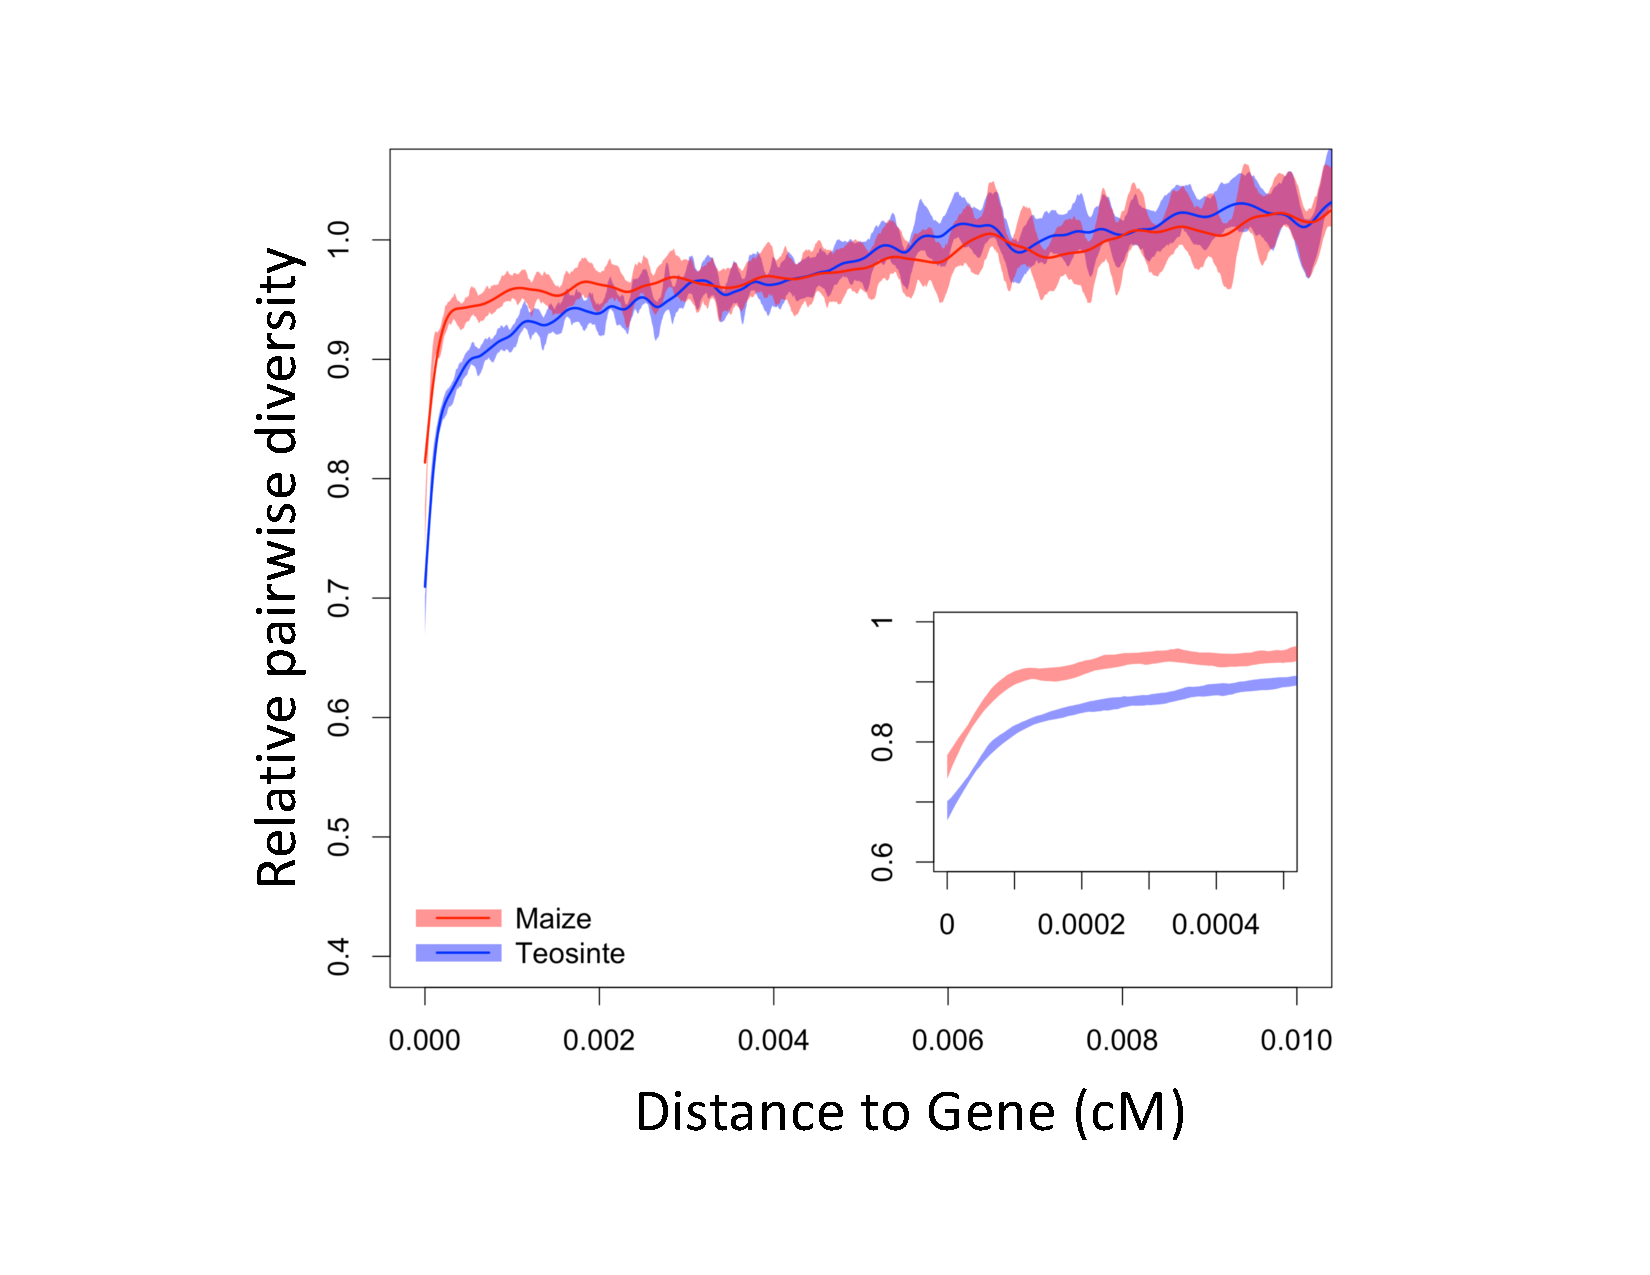
\includegraphics[width=\textwidth]{Journal_figs/recom_selection/maize_dist_gene/Figure4_beissinger_A.pdf}
\end{center}
\caption{Relative diversity compared to the mean diversity in windows
  $\ge 0.01$ cM as a function of the distance to the nearest gene.
  See \citep{beissinger2016recent} for details. Figure \PLOSccBY
   \href{https://github.com/RILAB/beissinger_ms}{ by Jeff Ross-Ibarra}.} \label{fig:BGS_maize}
\end{marginfigure}
More generally, if a neutral locus is surrounded by $L$ loci
experiencing purifying selection at recombination distances
$c_1,\cdots,c_L$, then compounding equation \eqref{eqn:pi_loc_BGS_1}
across these loci, the expected reduced diversity is approximately
\begin{equation}
\E[\pi] = \pi_0  \prod_{i=1}^L \left(1-\frac{\mu sh}{2(c_L+sh)^2}
\right) \approx \exp \left( \sum_{i=1}^L \frac{\mu sh}{2(c_i+sh)^2} \right) \label{eqn:pi_loc_BGS}
\end{equation}
To model an average neutral locus in a genomic region with a given recombination rate, we can imagine that our neutral locus is situated in the center of a large region with
total recombination rate $C$ and total deleterious mutation rate $U$,
where $U = \mu L$. Then our expression for diversity, equation \eqref{eqn:pi_loc_BGS}, simplies to 
\begin{equation}
\E[\pi] \approx \pi_0 \exp \left( \nicefrac{-U}{(sh+C)} \right)
\approx \pi_0 \exp \left( \nicefrac{-U}{C} \right). \label{eqn:GW_BGS_1}
\end{equation}
In this last approximation, we assume that we're looking at a
large region, with $C \gg sh$ . Note that much like genetic load,
equation \eqref{eqn:mut_load}, this expression depends only on the
total deleterious mutation rate. Any dependence on the selection
coefficient drops out, as weakly selected mutations segregate in the population at higher
frequencies, but are also removed from the population more slowly, allowing
more of the genome to recombine off the deleterious background. \\
\begin{marginfigure}[2cm]
\begin{center}
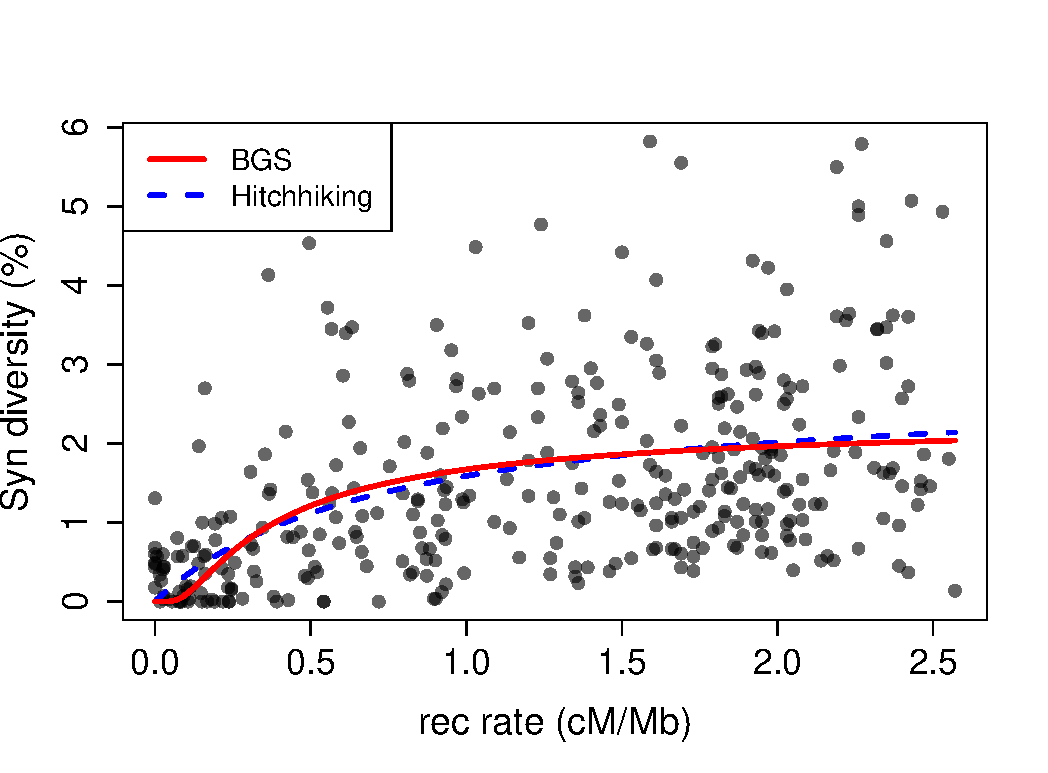
\includegraphics[width=\textwidth]{figures/Genomewide_BGS_HH.pdf}
\end{center}
\caption{The relationship between recombination rate and synonymous
  site pairwise diversity ($\pi$) in {\it D. melanogaster}, as
  in Figure \ref{fig:GW_hitchhiking_reduction}. The red curve is the
  predicted relationship between $\pi$ and recombination rate, obtained
  by fitting the BGS equation \eqref{eqn:GW_BGS_1} to this data  
 using non-linear least squares via the {\tt nls()} function in {\tt
   R}. The blue line is the recurrent hitchhiking equation line from Figure
 \ref{fig:GW_hitchhiking_reduction}. \gitcode{https://github.com/cooplab/popgen-notes/blob/master/Rcode/Genomewide_HH.R}} \label{fig:GW_BGS_reduction}
\end{marginfigure}

For a first go at fitting this to genome-wide data, we could look at
diversity in windows of length $W$ bp (as in Figure \ref{fig:GW_BGS_reduction}). If we assume that there is a constant rate of
deleterious mutation per base pair, $\mu_{BP}$, then $U=\mu_{BP}W$. Furthermore, if our genomic window has a
recombination rate $c_{BP}$ per base-pair, our total genetic length is
$R=c_{BP}W$. Making these substitutions in equation \eqref{eqn:GW_BGS_1}, our window size cancels out to give
\begin{equation}
  \E[\pi] \approx \pi_0 \exp \left(\nicefrac{-\mu_{BP}}{c_{bp}}
  \right) \label{eqn:GW_BGS_2}
 \end{equation}
Looking across windows that vary in their recombination rate,
i.e. $c_{BP}$, we can fit equation \eqref{eqn:GW_BGS_2} to data to
estimate $\mu_{BP}$. An example of doing this to data from {\it D. melanogaster}
  is shown in Figure
\ref{fig:GW_BGS_reduction}, yielding an estimate of the deleterious
mutation rate of $\mu_{BP}\approx
3.2 \times 10^{-9}$. This is roughly on the same order as the mutation
rate per base pair in  {\it D. melanogaster}, and so this deleterious mutation rate estimate is somewhat high as it
would require most of the genome to be constrained, but as a first
approximation it's not terrible. Note how similar the fit is to a model of
hitchhiking, suggesting that some combination of BGS and hitchhiking can explain the
broad relationship between diversity and recombination seen in {\it D. melanogaster} and other species.

%Our estimate
%of the deleterious mutation rate ($\mu_{BP}$) from the is too high again
%compatible with the idea that

\begin{figure}
\begin{center}
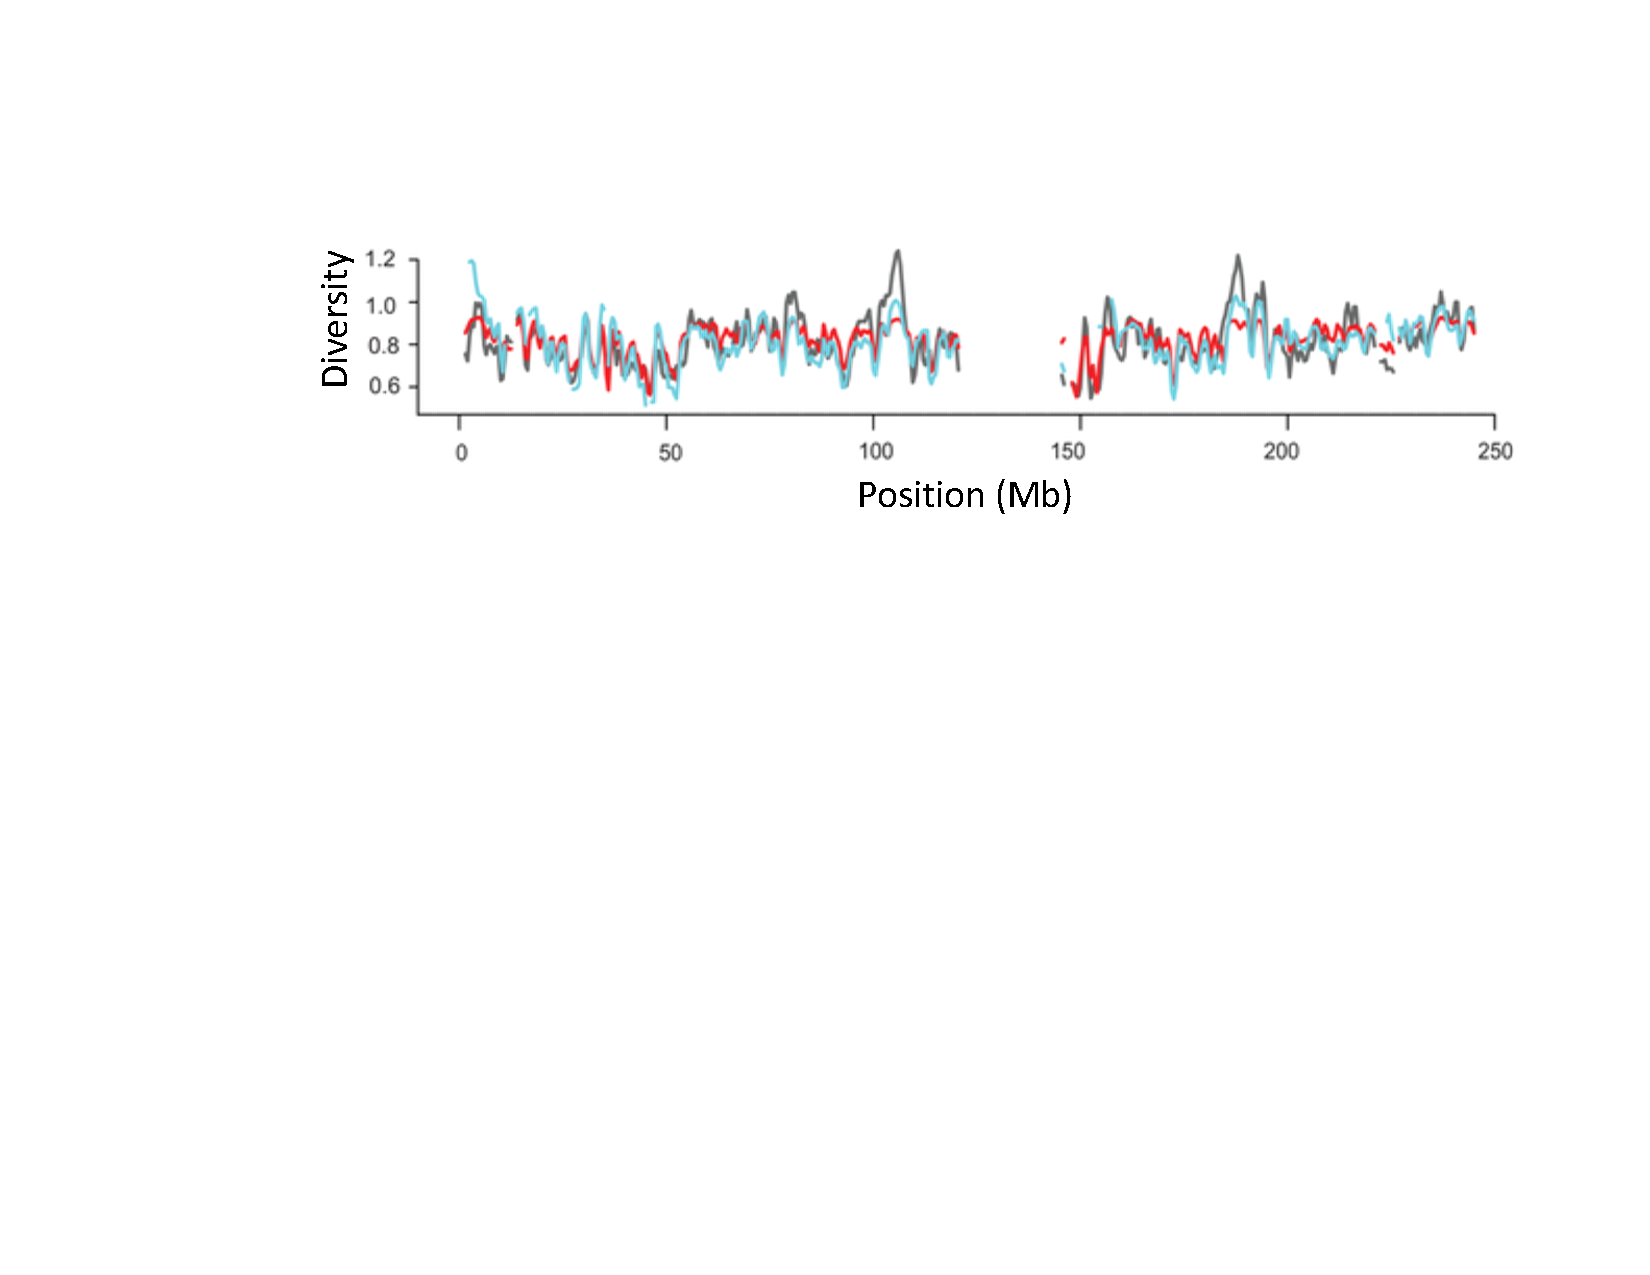
\includegraphics[width=\textwidth]{Journal_figs/recom_selection/McVicker_human_BGS/McVicker_human_BGS.pdf}
\end{center}
\caption{Observed (black line) and predicted pairwise diversity across
  chromosome 1, from a background selection model that assumes a
  uniform mutation rate (red line) or a mutation rate that varies with
  local human/dog divergence (blue line). Figure from
  \citep{Mcvicker:09}, \PLOSccBY. } \label{fig:McVicker_BGS}
\end{figure}

As our annotations of functional regions of the genome have improved, so have our
methods to infer background selection. A more rigorous version of this analysis today would incorporate variation in coding density among windows into the parameter $\mu_{BP}$. With detailed genomic annotations showing
coding regions and constrained non-coding regions, we can also move
beyond just analyzing broad-scale patterns. For example,
\citet{Mcvicker:09} fit a model of background selection to putatively
neutral pairwise diversity along the human genome, using equation
\ref{eqn:pi_loc_BGS} to estimate the effect of BGS at each locus,
weighing the genetic distance to all of the surrounding coding
regions and constrained non-coding sites. This allowed
\citet{Mcvicker:09} to estimate mutation rates and average selection
coefficients acting against deleterious alleles in these regions of
the genome. This best fitting model also allowed them to predict
diversity levels along the genome, a section of which is shown in
figure \ref{fig:McVicker_BGS}. Thus, broad-scale features of
polymorphism along the genome are well described by background selection
(or by linked selection more generally).

The deleterious mutation rates estimated by \citet{Mcvicker:09} from
fitting a model of BGS were again too high, as in the {\it Drosphila}
example above, suggesting the BGS alone is not sufficient to
explain all of the effect of linked selection. But how then do we go about distinguishing the impact of BGS from hitchhiking? 

\paragraph{Distinguishing the impact of hitchiking from  background selection in
  genome-wide data}

A variety of approaches have been taken to start to separate the effects of hitchhiking from background
selection. Much of the
strongest evidence showing the effects of both comes from
\textit{Drosophila melanogaster} and we review some of that evidence here. 
Hitchhiking is expected to have systematic effects on the neutral site
frequency spectrum, distorting it towards rare minor alleles,
(reflecting the slow recovery of diversity following a
sweep). Therefore, we should expect a distortion of summary
statistics such as Tajima's D in regions of low recombination if
hitchhiking is contributing to the reduction in diversity in these
regions \citep{Braverman:95, Przeworski:02,Kim:06}. In \textit{D. melanogaster}, there is a greater skew towards rare
alleles at putatively neutral sites in regions of low recombination
\citep{Andolfatto:01,Shapiro:07}; see left panel of Figure
\ref{fig:Tajimas_D_dN_pi}. However, while this skew isn't expected under
simple models of strong background selection.

\begin{figure}
\begin{center}
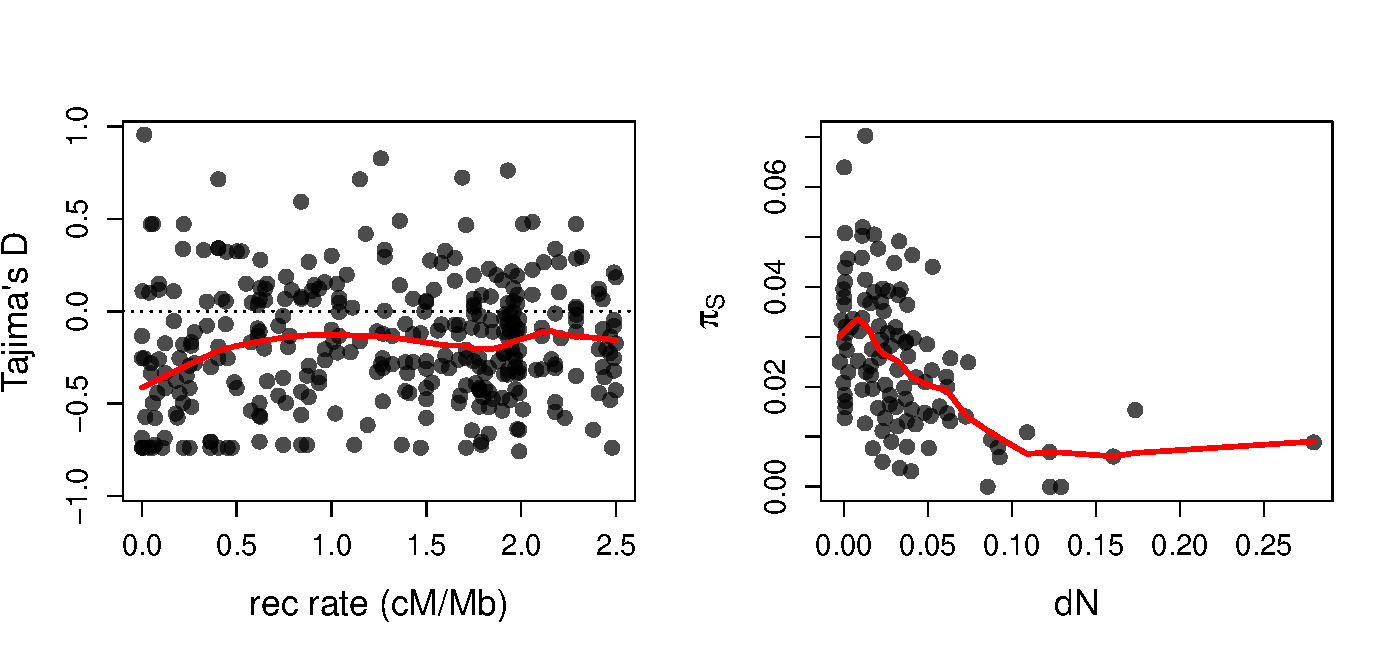
\includegraphics[width=\textwidth]{Journal_figs/recom_selection/Andolfatto_subs_vs_dN/Tajimas_D_subs_vs_dN.pdf}
\end{center}
\caption{{\bf Left)} Average Tajima's {\it D} in genomic windows plotted
  against their recombination rate in \textit{D. melanogaster}. Data
  from \citet{Shapiro:07}. {\bf Right)} Synonymous pairwise diversity
  in genomic windows  as a function of the density of non-synonymous
  subsitutions in the window. Data from \citet{Andolfatto:07}. \gitcode{https://github.com/cooplab/popgen-notes/blob/master/Rcode/Genomewide_HH.R}} \label{fig:Tajimas_D_dN_pi}
\end{figure}
\graham{Double check if Shapiro restricted the range on their recom rates}

Another prediction of the hitchhiking model, where an allele sweeps to
fixation, is that there should be a functional substitution associated with each
sweep. Or, to flip that around, we might expect to see a greater impact
of hitchhiking where there are more functional substitutions. 
For example, regions surrounding non-synonymous substitutions should have lower levels of
diversity, if a high fraction of non-synonymous substitutions are adaptive. Again, this pattern is seen in \textit{D. melanogaster}
\citep[][, right side of
Figure \ref{fig:Tajimas_D_dN_pi}]{Andolfatto:07, Macpherson:07,Sattath:11}.

\begin{figure}
\begin{center}
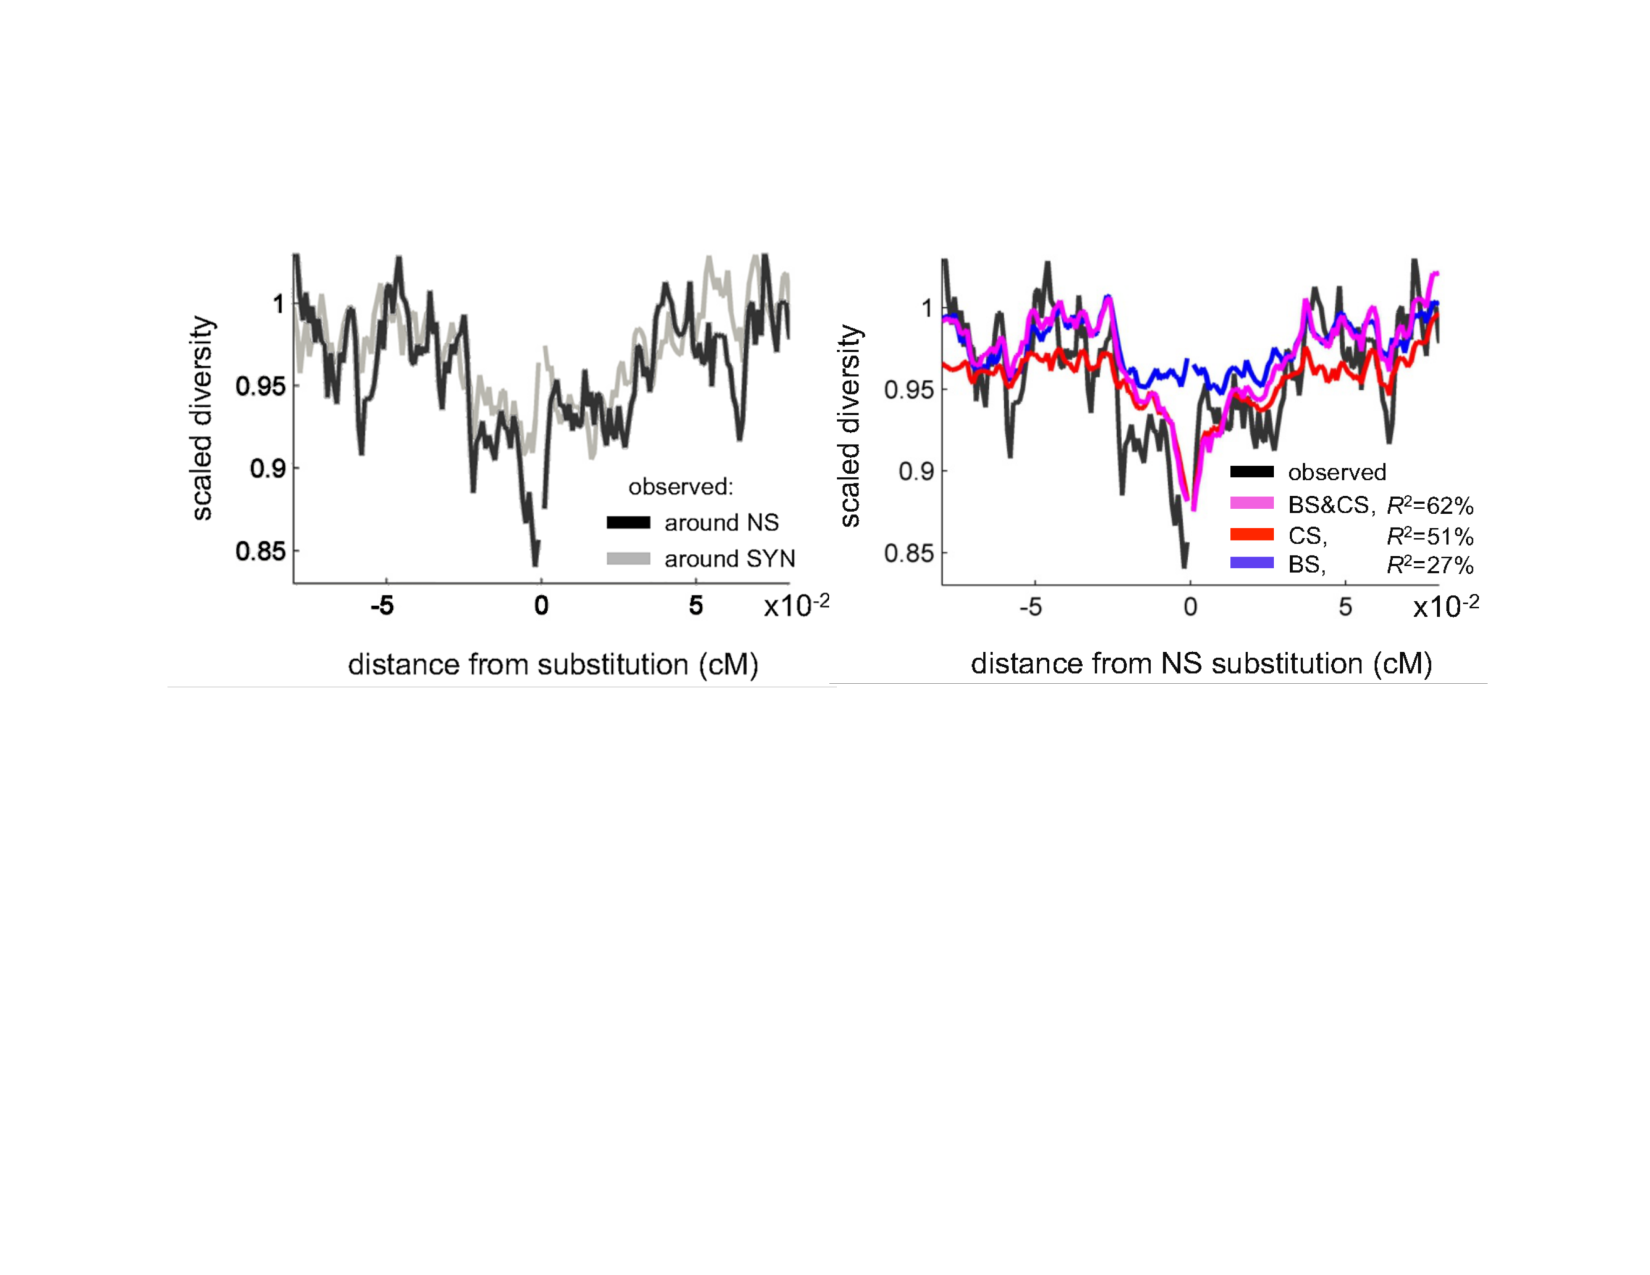
\includegraphics[width=\textwidth]{Journal_figs/recom_selection/Elyashiv_around_subs/Elyashiv_around_subs.pdf}
\end{center}
\caption{ {\bf Left) }  Scaled synonymous pairwise diversity levels around non-synonymous
  (NS) and synonymous (SYN) substitutions in {\it
    D. melanogaster}. {\bf Right)} Predicted scaled diversity levels
  around non-synonymous substitutions based on models including
  background selection (BS), classic sweeps (CS) and both (BS \&
  CS). Figure from \citet{elyashiv2016genomic}, \PLOSccBY.} \label{fig:Elyashiv_around_subs}
\end{figure}

Pushing this idea further, we can look at the dip in diversity
surrounding a non-synonymous substitution averaged across all the
substitutions in the genome. \citet{elyashiv2016genomic} found a
stronger dip in diversity around non-synonymous substitutions than
synonymous substitutions \citep[see also
][]{sattath2011pervasive}. Extending
the model of \citet{Mcvicker:09} to fit a model of background selection and
hitchhiking to putative neutral diversity along the genome, they found that
the dip in diversity around synonymous substitutions comes mostly from
BGS. But to fully explain the dip in diversity around non-synonymous
substitutions, a reasonable proportion of these non-synonymous
substitutions have to have been accompanied by a classic (hard)
sweep. The majority of these sweeps are estimated to be due to very
weak selection, with selection coefficients $<10^{-4}$. Furthermore, \citet{elyashiv2016genomic} estimated a
 $77$ - $89\%$ reduction in neutral diversity due to selection on linked sites, and concluded that no genomic window was entirely
free of the effects of selection. Thus linked selection has a profound
effect in some species such as {\it Drosophila melanogaster}. 



\section{Appendix. The probability of not recombining off the selected
  haplotype during the sweep.} \label{Appendix:no_recom_sweep}

We know that in the present day our neutral lineage is linked to
the selected allele. The probability that our lineage, in some
generation $t$ back in time, is in a heterozygote is $1-X(t)$, and the
probability that a recombination occurs in that individual is $r$. So
the probability that our neutral lineage is descended from a
recombinant haplotype $t$ generations back is 
\begin{equation}
c (1-X(t))
\end{equation}
So the probability ($p_{NR}$) that our lineage is not descended from a
recombinant haplotype 
from a recombination event in the
$\tau$ generations it takes our selected allele to move through the
population is
\begin{equation}
p_{NR}=\prod_{t=1}^{\tau} \big(1- c(1-X(j))\big)
\end{equation}
Assuming that $c$ is small, then $ \left(1- c(1-X(t))\right) \approx
e^{-r(1-X(t))}$,  such that
\begin{equation}
p_{NR}=\prod_{t=1}^{\tau} \left(1- c(1-X(t))\right) \approx \exp
\left( -c\sum_{t=1}^{\tau}
1- X(t) \right) =\exp
\left( -c \tau (1-\widehat{X}) \right)
\end{equation}
where
$\widehat{X}$ is the average frequency of the derived beneficial allele across its trajectory as it sweeps up in frequency,
$\widehat{X} = \frac{1}{\tau}  \sum_{t=1}^{\tau}
 X(t)$. As our allele is additive, its trajectory for frequencies
 $<0.5$ is the mirror image of its trajectory for frequencies $>0.5$, therefore its
average frequency $\widehat{X} =0.5$. This simplifies our expression to
\begin{equation}
p_{NR} = e^{-c \tau/2 }.
\end{equation}



\begin{ChapterSummary}
\item When an initially rare selected allele sweeps up in frequency it carries with it the genetic background (haplotype) that it arose on. Alleles that are lucky enough to hitchhike along with the
  selected allele are dragged to high frequency and diversity is depleted by this hitchhiking effect.
\item In recombining regions, diversity is only locally supressed by a selective sweep as further from the selected site alleles can recombine on/off of the sweep allowing diversity to persist in the population. The genomic scale of the hitchiking effect depends linearly on the time it take the selected allele to sweep through the population and inversely on the local recombination rate. The characteristic dip in diversity is used to find selective sweeps in genome scans and to estimate the timing and strength of selection. 
\item Selective sweeps leave a range of other genomic signals that have been used to identify them, including distortions to the frequency spectrum (a more extreme skew towards rare alleles) and elevated $F_{ST}$ between populations.
\item We see reduced diversity in regions of low recombination consistent with the greater removal of diversity in these regions due to recurrent hitchhiking. However, this genome-wide effect is also consistent with background selection, the removal of linked diversity along with deleterious alleles. 

\end{ChapterSummary}

\begin{marginfigure}
\begin{center}
  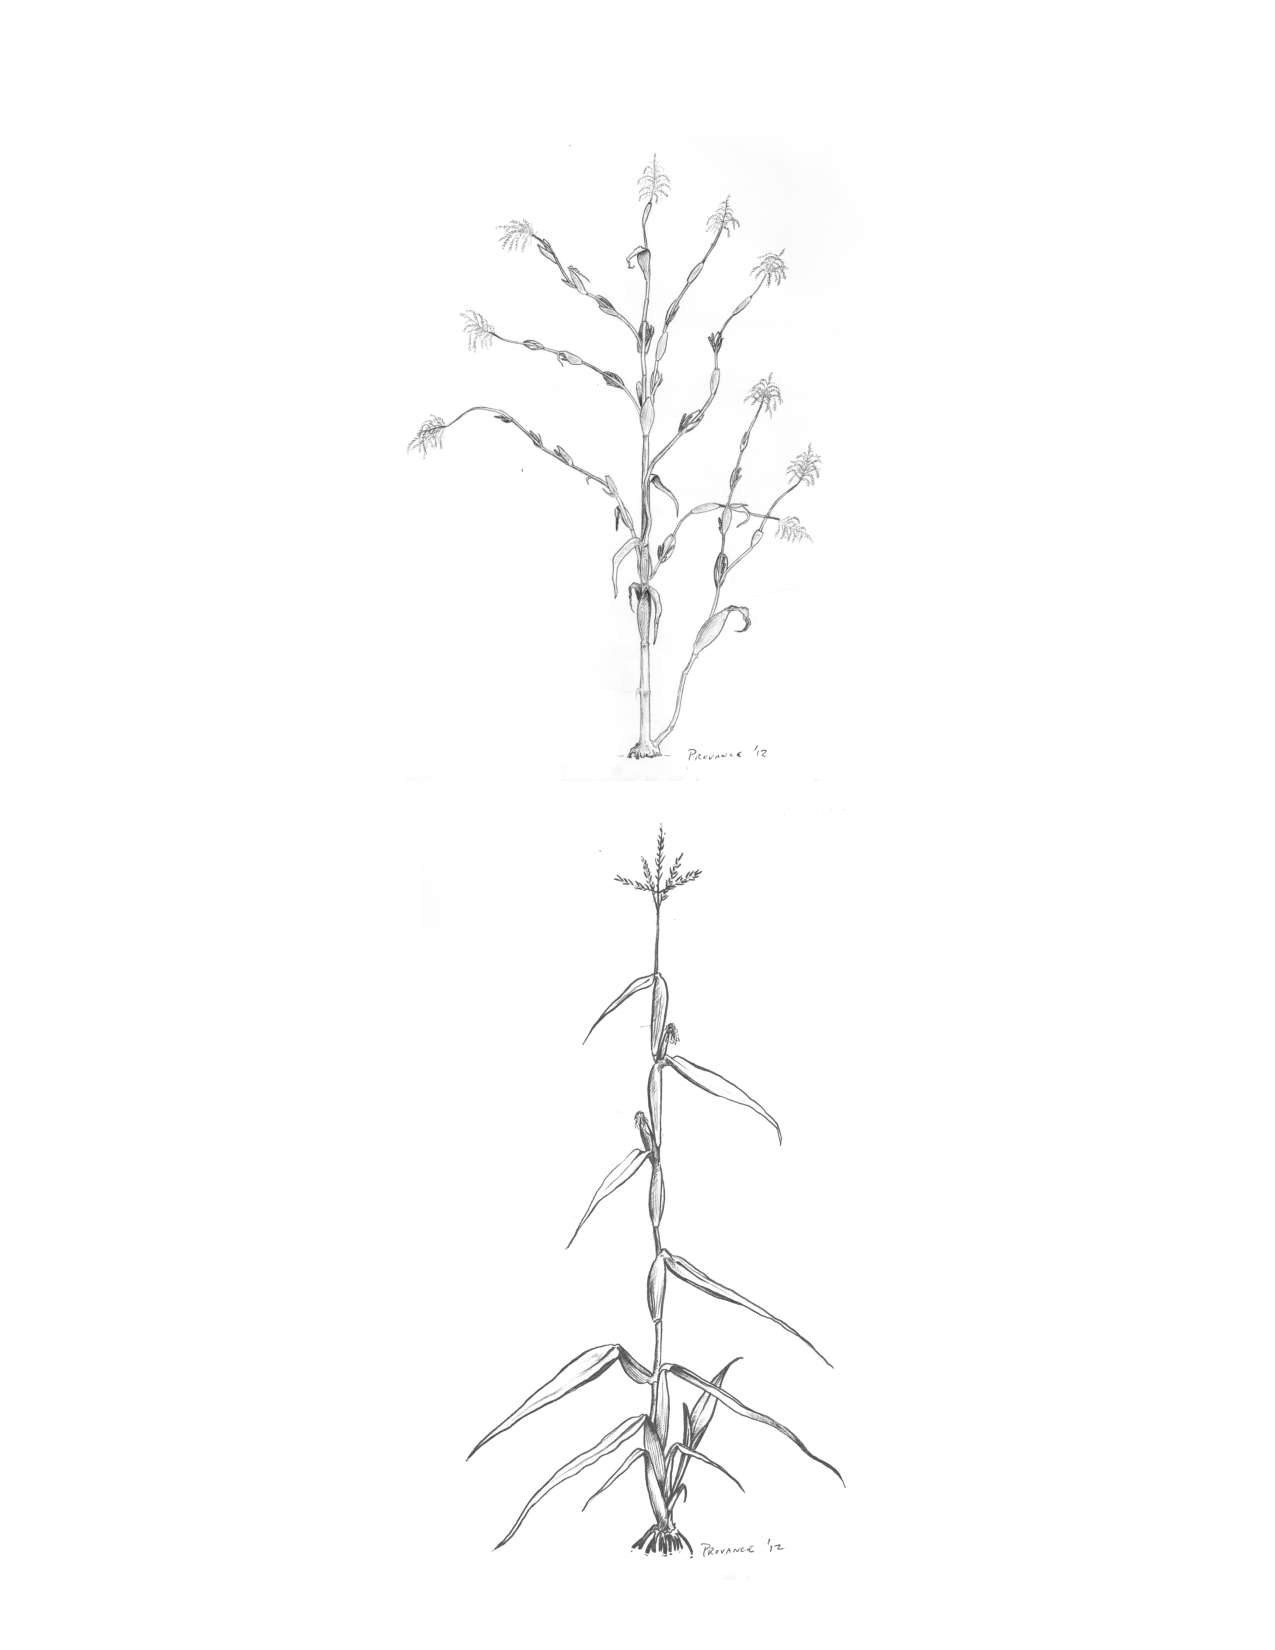
\includegraphics[width = \textwidth]{illustration_images/hitchhiking/maize_teosinte/maize_teosinte_tall.pdf}
\end{center}
\caption{{\bf Top)} Teosinte plant architecture is branched, with
  multiple ears per plant. {\bf Bottom)} Maize architecture is apically dominant, with side branches tipped by female inflorescences
(ears) Caption and image (cropped) from \citet{stitzer2018maize} drawn
by Mitchell Provance. \PLOSccBY. } \label{Fig:branched_teosinte} %% figure in
                                %% ILS_ABBA_BABA power point
\end{marginfigure}

\begin{question}{}
  Modern maize derived from teosinte, a weedy plant that grows in South and
  Central America. A striking phenotypic difference between teosinte and maize
  is that teosinte is a bushy plant, while maize grows primarily upwards. One
  gene that has been implicated in this transformation is tb1. \citet{wang1999limits} sequenced a region around this
  gene to find that background levels of neutral diversity decrease around this
  gene.\\

{\bf A)} It takes roughly 300bp for the diversity to recover moving
away from the sweep.  \citeauthor{wang1999limits} estimate
$r = 4 \times 10^{-7}$ per base pair. Estimate the time (in years) since the selected maize
variant of tb1 arose as a new mutation. Maize is an annual plant, so assume 1
generation per year.\\
{\bf B)} Assume that the effective size of this diploid population is $N = 10^6$. What is the selective
coefficient of this tb1 allele?
\end{question}

%For strongly deleterious alleles, this continuous loss acts primarily
%to increase the variance of  at markers closely linked to loci with high deleterious mutation rates \citep{Hudson:95b,Nordborg:96}. Therefore, this background selection model leads to a reduction in genetic diversity but no skew in the frequency spectrum. However, a skew towards rare neutral alleles can result if weakly deleterious mutations are incorporated into the model \citep{Nordborg:96, Gordo:02}.